% !TEX encoding = UTF-8 Unicode
\documentclass[twoside]{supsistudent} 

\graphicspath{ {images/} }
\restylefloat{table}
% per settare noindent
\setlength{\parindent}{0pt}

\colorlet{punct}{red!60!black}
\definecolor{background}{HTML}{EEEEEE}
\definecolor{delim}{RGB}{20,105,176}
\colorlet{numb}{magenta!60!black}

\lstdefinelanguage{json}{
    basicstyle=\normalfont\ttfamily,
    numbers=left,
    numberstyle=\scriptsize,
    stepnumber=1,
    numbersep=2pt,
    showstringspaces=false,
    breaklines=true,
    frame=lines,
    backgroundcolor=\color{background},
    literate=
     *{0}{{{\color{numb}0}}}{1}
      {1}{{{\color{numb}1}}}{1}
      {2}{{{\color{numb}2}}}{1}
      {3}{{{\color{numb}3}}}{1}
      {4}{{{\color{numb}4}}}{1}
      {5}{{{\color{numb}5}}}{1}
      {6}{{{\color{numb}6}}}{1}
      {7}{{{\color{numb}7}}}{1}
      {8}{{{\color{numb}8}}}{1}
      {9}{{{\color{numb}9}}}{1}
      {:}{{{\color{punct}{:}}}}{1}
      {,}{{{\color{punct}{,}}}}{1}
      {\{}{{{\color{delim}{\{}}}}{1}
      {\}}{{{\color{delim}{\}}}}}{1}
      {[}{{{\color{delim}{[}}}}{1}
      {]}{{{\color{delim}{]}}}}{1},
}

% Crea un capitolo senza numerazione che pero` appare nell'indice %
\newcommand{\problemchapter}[1]{%
  \chapter*{#1}%
  \addcontentsline{toc}{chapter}{#1}%
\markboth{#1}{#1}
}

% Numerazione delle appendici secondo norma
\addto\appendix{
\renewcommand{\thesection}{\Alph{chapter}.\arabic{section}}
\renewcommand{\thesubsection}{\thesection.\arabic{subsection}}}

\setcounter{secnumdepth}{5} 	%per avere più livelli nei titoli
\setcounter{tocdepth}{5}		%per avere più livelli nell'indice


\titolo{Viki: Smart Home Natural Language Interface }
\studente{Luca Ambrosini}
\relatore{Nicola Rizzo}
\correlatore{Alan Ferrari}
\committente{-}
\corso{-}
\modulo{M00002 Progetto di diploma}
\anno{2015/16}

\begin{document}

\pagenumbering{alph}
\maketitle
\onehalfspacing
\frontmatter

%	Indici vari

\pagenumbering{roman}
\tableofcontents
\listoffigures					
\listoftables					

\newpage
\mainmatter
\pagenumbering{arabic}
\setcounter{page}{1}
\problemchapter{Abstract}
Le interfacce in linguaggio naturale permettono all’utente di controllare un sistema attraverso la voce. Esse sono estremamente efficaci, ma vengono spesso criticate per la loro rigidità.\\
I metodi generalmente utilizzati per la costruzione di queste interfacce sono basati su un sistema di regole, dette grammatiche fisse, alle quali l’utente si deve attenere per l’interazione.\\
Il sistema introduce una nuova metodologia di associazione delle frasi pronunciate dall’utente ai comandi disponibili nella casa, questo avviene attraverso l'astrazione delle parole in vettori e alla comparazione di essi; senza l'ausilio di un sistema di regole.\\
Il sistema è sempre in ascolto e viene attivato alla la pronuncia del suo nome, inoltre è predisposto per l’apprendimento di nuovi comandi, insegnati vocalmente dall’utente.\\
L’assenza di grammatiche e la possibilità di insegnamento garantiscono una maggior flessibilità, rendendo la conversazione con l’Agente più simile ad una conversazione reale.\\
La lingua scelta per la realizzazione è l’inglese, ma è possibile aggiungere ulteriori lingue.\\
\problemchapter{Progetto assegnato}
\section*{Descrizione}
Nell'ambito della home automation è possibile sviluppare Interfacce Utente sempre più sofisticate e complesse; quelle più interessanti e facilmente utilizzabili sono però le cosiddette NUI, Natural User Interfaces: esse devono cercare di "sparire" e nascondere la complessità del sistema sottostante alla percezione dell'utente.In questo contesto assume particolare importanza il riconoscimento vocale, in grado di liberare l'utente dall'interazione fisica con i dispositivi: basti pensare ad applicazioni di tipo medicale o in situazioni in cui un utente disabile, anziano o con problemi di salute non è in grado di utilizzare in maniera tradizionale un sistema domotico.

Il Laboratorio di Internet of Things dell'Istituto Sistemi Informativi 
e Networking del DTI dispone di un ambiente
domotico controllato da una NUI basata su riconoscimento vocale; 
attualmente il sistema di riconoscimento è basato su
grammatiche fisse. Ciò significa che l'utente non può esprimersi 
scegliendo liberamente le parole da usare, ma deve
pronunciare delle frasi prestabilite,
 pur sempre limitate per quanto numerose.
Si vuol realizzare sulla infrastruttura presente un modulo
 software che permetta di superare le limitazioni correnti.
\section*{Compiti}
Si richiede che lo studente sviluppi uno o più moduli che:
\begin{itemize}
\item riconoscano con continuità quello che l'utente sta dicendo
\item siano in grado di eseguire una analisi semantica (dipendente dalla lingua) 
sul testo in uscita dal punto precedente
\item possano capire se la richiesta effettuata è valida o meno nel contesto 
corrente, una volta letto lo stato del
sistema.
\item In caso affermativo, dovrà passare la richiesta al sistema esistente 
per controllare i dispositivi collegati
\item Attendere eventualmente l'esito della richiesta e riportarlo all'utente 
nel modo migliore (tipicamente text to speech)
\end{itemize}
\section*{Obbiettivi}
\begin{itemize}
\item Studiare il sistema domotico esistente nel laboratorio e comprenderne i meccanismi di funzionamento
\item Approfondire la conoscenza della Internet of Things
\item Apprendere meccanismi di NLP (Natural Language Processing)
\item Far comunicare sistemi eterogenei scritti con tecnologie differenti
\end{itemize}
\section*{Tecnologie}
\begin{itemize}
\item riconoscimento vocale, grammatiche, NLP
\item c\# e .net Framework
\item Web servers
\item EcmaScript5 / 6 e Node.js
\item Sockets e websockets
\end{itemize}
%	Inizio Documento
\chapter{Introduzione}

Disegnare una macchina in grado di comportarsi come un umano, in particolare di parlare e interpretare il linguaggio, è uno degli obbiettivi dell'Ingegneria sin da metà del 20esimo secolo. Le interfacce in linguaggio naturale sono considerate come il punto di arrivo dell'interazione uomo macchina.
Lo sviluppo in questo campo è stato molto intenso negli ultimi anni, ciò ha permesso la realizzazione di agenti intelligenti che simulino una conversazione e che riescano a compiere azioni più complesse di semplici comandi con frasi standardizzate.

\section{Cenni storici}

Il primo esempio nella storia di dispositivo ad interazione vocale è da collocare nell'estate del 1952, presso i laboratori Bell.
Quell' vennero eseguiti i primi test di "Audrei" (Automatic Digit Recognizer), un dispositivo in grado di comporre un numero di telefono dettato ad un microfono.

Nel 1962 IBM presentò "Shoebox", una macchina in grado di comprendere 16 diverse parole pronunciate in inglese. Questa macchina era destinata ad essere una calcolatrice vocale.

Lo sviluppo di sistemi in grado di comprendere il linguaggio naturale è poi proseguito nel tempo, passando dalla comprensione di pochi suoni alla comprensione continua del linguaggio; le tecniche si sono evolute passando da metodi statistici fino ad approcci basati sul deep learning. Esso è una branca del machine learning, che simula delle reti neurali multi strato che riescono ad apprendere funzioni complesse. \cite{deeplearninggeneral}

Grossi miglioramenti in questo campo sono pervenuti nell'ultimo secolo, soprattuto grazie all'incremento delle capacità computazionali. Questo ha permesso la realizzazione di agenti intelligenti sempre più complessi.

\section{Evoluzione degli agenti}

I primi dispositivi ad interazione vocali sono stati gli "Interactive Voice Response", cioè gli agenti dei call center, che descrivevano attraverso la voce i comandi e ricevevano input attraverso i numeri digitati sul telefono. Il numero di input era quindi molto ridotto e la struttura della conversazione era fissa.

Successivamente i lettori automatici e i dispositivi ad interazione vocale sono stati integrati nei sistemi operativi. La loro funzione principale consisteva nell'aiutare le persone con delle disabilità. Era comunque necessario un microfono, quindi una prossimità al computer. Inoltre la voce aveva una funzione di sostituzione delle capacità visive o motorie; non erano previste funzionalità dedicate che permettessero una maggior produttività.

Con gli smartphone, che sono dotati di un microfono e che dispongono di una connessione a Internet, gli agenti intelligenti sono diventati parte della nostra vita quotidiana. Vista la limitata capacità di calcolo degli smartphone tutto il processamento dell'informazione viene eseguito attraverso cloud computing.\\
L'ultima generazione è costituita da dispositivi da interazione vocale come "Amazon Alexa" e "HAL", essi sono in grado di ricevere input vocali in modo continuo, senza che l'utente debba avere un microfono appresso e senza che sia necessario azionare un dispositivo. Questo ha portato l'interazione vocale ad un nuovo livello di usabilità e ha aperto nuove possibilità di utilizzo di questa tecnologia, in particolare nell'ambito delle smart home.\cite{alexa}\cite{HAL}

\section{Il momento giusto}

Storicamente lo scetticismo a proposito delle interfacce in linguaggio naturale è sempre stato molto elevato: soprattuto per la loro scarsa produttività sono sempre state considerate un accessorio e non una tecnologia che potesse essere sfruttata.
Ora però tutte le tecnologie necessarie alla realizzazione di un agente intelligente che ci possa aiutare nella vita quotidiana sono pronte:
\begin{itemize}
  \item \textbf{Speech To Text:} Grazie alle tecniche di machine learning sviluppate negli ultimi anni, questa tecnologia è arrivata ad alti livelli di accuratezza, superando in alcuni casi perfino le capacità di percezione dell'uomo. Sono ormai disponibili servizi che eseguono speech-to-text in tutte le lingue del mondo.\cite{sttmachinelearning}
  \item \textbf{Comprensione del testo:} L'analisi semantica e la vettorizzazione di parole e frasi permettono una sempre maggior strutturazione del contenuto del testo, la quale consente una migliore comprensione da parte delle macchine.\cite{word2vec}
  \item \textbf{Connessione:} La capacità di calcolo richiesta per effettuare la trascrizione del testo e per la sua comprensione è molto elevata, per questo in genere si ricorre a un server remoto; l'incremento della larghezza di banda e la diminuzione dei tempi di latenza hanno reso possibile delle risposte in tempi adeguati.
  \item \textbf{Audio always on:} La tecnologia ha permesso la creazione di dispositivi che ascoltano in modo continuo e sono in grado di riconoscere delle keyword per la loro attivazione (es. "Ehi Siri"); le persone inoltre si sono abituate e hanno imparato ad accettare questa invasione della privacy.
  \item \textbf{IOT:} Si stima che il mercato dell'IOT raggiunga una cifra d'affari di 6200 Miliardi di \$ entro il 2025 e l'home automation è uno dei settori nei quali un agente può raggiungere la sua massima utilità.\cite{IOTGeneral}
\end{itemize}

\chapter{Caso d'uso}

L'utilità degli agenti intelligenti ad interazione vocale è spesso messa in dubbio, ma ci sono alcune occasioni nelle quali le loro capacità brillano, poiché forniscono un'esperienza d'uso diversa dalle interfacce basate su display o touchscreen:
\begin{itemize}
	\item \textbf{Accessibilità}: Consentono un'esperienza d'uso soddisfacente a persone con disabilità motorie o visive, in quanto la procedura di descrizione delle operazione possibili e la successiva richiesta di un input non è più necessaria, gli agenti possono infatti eseguire comandi in risposta a frasi come "Manda un messaggio a Mario dicendo che arriverò tardi"
	\item \textbf{Eye-busy o Hand-busy}: In scenari quali la guida o attività svolte in cucina, in cui si hanno le mani impegnate e non si ha la possibilità di concentrare la propria attenzione su uno schermo, gli agenti intelligenti diventano particolarmente utili.
	\item \textbf{Automazione casalinga}: Supportare la creazione di comandi complessi a discrezione dell'utente, che permettano di compiere azioni in modo semplificato. Ad esempio "Buonanotte" potrebbe automaticamente abbassare tutte le tapparelle e spegnere tutte le luci.
\end{itemize}
In queste situazioni sarebbe quindi ideale avere un agente in grado di svolgere per noi la maggior parte delle operazioni che gli vengono indicate attraverso la voce, come se stessimo conversando con una persona alla quale chiediamo di svolgere il compito.

\chapter{Obiettivo}

Il progetto è basato su "Viki", un agente intelligente, capace di controllare molti degli apparecchi presenti in un abitazione e di fornire informazioni, ad esempio riguardanti il meteo.\cite{agenteinteligente}
Esso è stato sviluppato presso l'Istituto Sistemi Informativi e Networking. \cite{ISIN}
Il primo obbiettivo del progetto di bachelor consiste nella comprensione dell'infrastruttura del sistema attuale; successivamente si  vuole migliorare l'interazione vocale con il sistema, cercando di renderla il meno rigida possibile. Inoltre si implementeranno strutture atte a migliorare l'intelligenza dell'agente.

\section{Interfaccia in linguaggio naturale}
\subsection{Grammatiche fisse}
Il sistema attuale prevede l'interazione vocale, ma utilizza un sistema basato su delle grammatiche fisse. Questo implica quindi una struttura della frase definita a priori dal programmatore, che nel caso non sia rispettata, impedisce la comprensione del comando da parte dell'Agente.
\subsection{Rimozione dei vincoli}
Il progetto aspira a creare un'interfaccia libera da questi vincoli, che provi a comprendere il senso della frase in modo indipendente dai singoli vocaboli e dalla struttura utilizzata.\\
Grazie all'interfaccia libera l'utilizzatore può concentrarsi sull'azione da eseguire e meno su come esprimerla per far sì che l'Agente sia in grado di comprenderla. Una delle critiche che viene più spesso mossa alle interfacce in linguaggio naturale è la necessità dell'utilizzatore di compiere uno sforzo mentale per pensare come la macchina.
Grazie alla rimozione di questi vincoli l'utilizzatore dovrebbe trovare l'interazione con l'agente più simile a una conversazione tra persone, garantendo quindi una maggior soddisfazione.
Un'interfaccia di questo livello semplificherebbe l'utilizzo di una smart home al punto di renderla fruibile anche a persone che non si trovano normalmente a loro agio con la tecnologia.
\section{Incremento delle API}
\subsection{API attuali}
Le capacità del sistema sono strettamente collegate alla mole di informazioni alle quali esso ha accesso e ai dispositivi che è in grado di controllare. 
Al momento Viki può controllare :
\begin{itemize}
  \item Lampadine philips HUE (accensione, colorazione, intensità)
  \item Prese di corrente z-wave (accensione, lettura potenza istantanea)
\end{itemize}
e ha accesso alle seguenti informazioni:
\begin{itemize}
  \item Sensori di movimento, luminosità, umidità, temperatura
  \item Previsioni meteo (yahoo)
\end{itemize}
\subsection{API future}
Durante lo sviluppo del progetto di bachelor si vogliono incrementare le capacità del sistema, in particolare Viki dovrà essere in grado di controllare:
\begin{itemize}
  \item Tapparelle motorizzate
  \item Mediacenter
  \item Impostazione di sveglie
  \item Impostazione di promemoria
  \item Aggiunta eventi calendario
  \item Impostazioni timer
\end{itemize}
e avrà accesso a informazioni aggiuntive quali :
\begin{itemize}
  \item Palinsesto televisivo (RSI, Mediaset, Rai)
\end{itemize}

\chapter{Stato dell'arte}

In questo momento storico numerosi sforzi si stanno concentrando per la creazione di interfacce in linguaggio naturale, con particolare interesse nell'ambito dell'IOT  e dell'automazione casalinga. 

Sono presenti sul mercato diversi software che svolgono compiti simili, alcuni di essi sono open-source, mentre altri sono software commerciali; in questo capitolo verranno confrontate le funzionalità di quanto implementato con i principali prodotti software commerciali.
\section{Prodotti commerciali}
\subsection{Google, Amazon, Apple}
Molti dei grandi produttori, come Google, Amazon e Apple, stanno per rilasciare o hanno già sviluppato i loro agenti intelligenti. \cite{googleAgent}\cite{homekit}\cite{alexa}

Essi garantiscono una modalità di ascolto always-on e riescono a comprendere frasi indipendentemente dalla loro sintassi, ma richiedono che i devices siano accessibili dall'esterno attraverso il web. Inoltre la computazione avviene attraverso il cloud, è quindi necessaria una connessione a internet sempre attiva.
Gli agenti di questi produttori offrono delle API di livello molto alto, non è quindi evidente l'integrazione con un sistema come quello di partenza utilizzato nel progetto.

\subsection{HAL}
Alcune aziende nell'ambito dell'automazione casalinga hanno integrato i loro prodotti con un'interfaccia in linguaggio naturale, ad esempio HAL. Questi prodotti commerciali hanno dei costi elevati e le licenze pongono delle limitazioni a proposito dei dispositivi che possono essere controllati. Il prodotto analizzato inoltre necessità di personale qualificato che provveda alla completa installazione dei sistema, che non può in seguito essere modificata dall'utente.\cite{HAL}

\section{Prodotti open-source}
Il principale prodotto open-source per costruire un interfaccia in linguaggio naturale è Jasper; esso permette di definire azioni che devono essere eseguite in risposta a determinati input vocali. \cite{jasper}

Il prodotto funziona in locale, non necessita di una connessione a Internet ed è facilmente integrabile in un ambiente esistente, però sia la funzionalità di speech to text che l'associazione frase-comando vengono eseguite attraverso un sistema di regole predefinite; come avviene nel sistema attuale.

Questi vincoli limitano l'esperienza d'uso, in quanto l'utente deve conoscere esattamente una delle frasi necessarie all'invocazione di un comando per poterlo far eseguire dalla casa.



\section{Viki}
Il prodotto realizzato si differenzia dai prodotti commerciali per i seguenti motivi:
\begin{itemize}
	\item \textbf{Indipendenza da Internet}: Rispetto alla gran parte dei software commerciali la maggior parte del processamento viene effettuata offline. Integrando un API locale di speech to text il software potrebbe funzionare senza l'accesso a Internet.
	\item \textbf{Devices locali}: Non è richiesto che i devices controllati dal sistema siano esposti il rete, la loro gestione è effettuata attraverso i driver nel sistema. Sono quindi evitati problemi di privacy e sicurezza.
\end{itemize}
Viki inoltre si diversifica dai principali prodotti open-source per i seguenti motivi :
\begin{itemize}
	\item \textbf{Convention over configuration}: L'interfaccia in linguaggio naturale è stata sviluppata appositamente per il sistema già esistente, non è quindi necessario gestire configurare il sistema in quanto tutte le informazioni vengono estratte automaticamente dal codice. Nel caso alcune informazioni volessero essere gestire manualmente dall'utente è possibile annotare i metodi che eseguono le operazioni.
	\item \textbf{STT generico}: Il modulo di trasformazione non è basato su un sistema di regole, il sistema è quindi in grado di trasformare \(quasi\) tutti i vocaboli in testo
	\item \textbf{Indipendente da vocaboli e sintassi}: i principali sistemi sono basati su sistemi di regole ai quali i comandi devono sottostare per poter essere compresi. Le regole impongono sia una sintassi che l'utilizzo di determinati vocaboli. Attraverso l'astrazione di parole in vettori Viki riuscirà ad essere indipendente dai vocaboli e dalla sintassi usata nella frase.
\end{itemize}
Infine il sistema sviluppato si differenza dai prodotti attualmente disponibili per la seguente funzionalità:
\begin{itemize}
	\item \textbf{Apprendimento di comandi}: Attraverso l'interfaccia vocale è possibile insegnare dei nuovi modi per invocare comandi del sistema. Il sistema è quindi in grado di imparare espressione gergali, migliorando con il passare del tempo.
\end{itemize}
\chapter{Architettura}
Il sistema sviluppato durante il progetto di bachelor si compone di diversi moduli:
\begin{itemize}
	\item \textbf{Ears}: Riconosce la keyword di inizio conversazione, trasforma in testo quanto detto dall'utente. (Python)
	\item \textbf{Brain}: Trasforma il testo ricevuto dal componente Ears in un comando, che viene comunicato a Engine. Si occupa inoltre di modificare lo stato della conversazione di Ears. (Java)
	\item \textbf{GUI}: Alternativa a Voice e Ears, sviluppata principalmente per motivi di debug. (Electron)
	\item \textbf{Voice}: Notifica all'utente quando un comando viene eseguito, quando non viene compreso e gli pone domande se necessario. (Python)
	\item \textbf{Engine}: Comunica a Brain quali comandi offre ed esegue i comandi ricevuti. (NodeJs)
\end{itemize}
\begin{figure}[H]
\centering
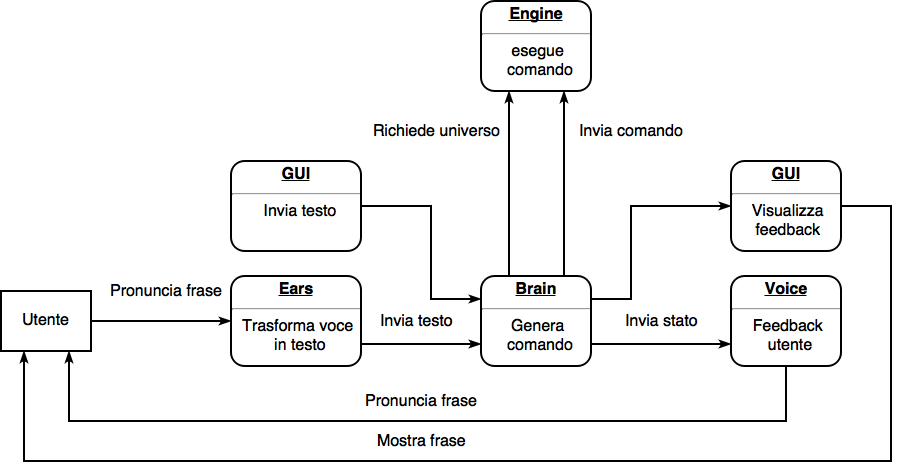
\includegraphics[width=\textwidth]{Architettura}
\caption{Architettura del sistema}
\label{fig:pose}
\end{figure}
\section{Vantaggi}
Si è scelto di separare il sistema in diverse componenti per favorirne la riutilizzabilità. Si è cercato di ridurre al minimo le interdipendenze, cercando di rendere ogni componente autonomo e riusabile in altri contesti.

Motivazione principale per la separazione in componenti è stata la maggior libertà tecnologica, infatti i vari moduli sono realizzati in linguaggi diversi. 
Questa scelta ha consentito utilizzo del linguaggio per il quale era disponibile la miglior libreria.

\section{Svantaggi}

La separazione in moduli ha però richiesto uno sforzo superiore alla realizzazione di un singolo componente, in quanto è stato necessario creare degli appositi canali di comunicazione si è inoltre resa necessaria la definizione di formalismi per la trasmissione dell'informazione.

Infine la trasmissione su di un canale è più onerosa e lenta rispetto alla condivisione dello stesso spazio di memoria, ma per la quantità di dati che è necessario trasmettere questa differenza non è stata ritenuta significativa.

\chapter{Comunicazione tra componenti}
I diversi canali di comunicazione hanno esigenze diverse, abbiamo quindi utilizzato tecnologie diverse a seconda del canale.

\section{Engine-Brain}
Brain deve essere informato da Engine a proposito di quali sono i comandi che possono essere eseguiti, quest'operazione avviene una sola volta durante la fase di inizializzazione del sistema.

L'informazione viene reperita da Brain, seguendo l'architettura REST, attraverso una chiamata all'indirizzo GET \textit{"/metadata"}, all'indirizzo di Engine. Essa ritorna una struttura dati JSON che descrive le capacità il sistema, seguendo il formalismo documentato nel capitolo apposito.
\section{Altre comunicazioni}
I canali di comunicazione Ears-Brain e Brain-Engine vengono utilizzati ad ogni interazione con l'utente, per questo motivo si è deciso di non seguire l'architettura REST, ma di utilizzare dei canali di comunicazione di tipo websocket.

Per la realizzazione di questo tipo di canale è stata scelta la tecnologia socket.io. 
\subsection{Socket.io}
Socket.io si occupa di creare un canale di trasmissione che una comunicazione bi-direzionale; essa si basa sull'emissione di eventi che possono essere divisi in categorie attraverso l'utilizzo dei namespace.

Questa tecnologia garantisce un livello di astrazione dalla tecnologia di trasporto utilizzato. Inoltre si occupa di gestire autonomamente il failover : quando il client o il server non sono disponibili, i messaggi vengono messi in coda e verranno inviati alla riconnessione del dispositivo.

Questa tecnologia è stata scelta anche per la disponiblità di implementazioni in tutti i linguaggi utilizzati:
\begin{itemize}
	\item \textbf{Python client}: https://pypi.python.org/pypi/socketIO-client
	\item \textbf{Python server}: https://github.com/miguelgrinberg/python-socketio
	\item \textbf{Nodejs client}: https://www.npmjs.com/package/socket.io-client
	\item \textbf{NodeJs server}: https://www.npmjs.com/package/socket.io
	\item \textbf{Java client}: https://github.com/socketio/socket.io-client-java
	\item \textbf{Java server}:https://github.com/mrniko/netty-socketio
\end{itemize}

\chapter{Comunicazione Ears - Brain }
Brain possiede una struttura che permette l'utilizzo di canali di comunicazione input. Nell'implementazione attuale i comandi vengono ricevuti attraverso un socket server esposto sulla porta 8887.
\section{Input}
Su questo canale possono pervenire messaggi qualificati dal namespace "textCommand", l'oggetto trasmesso nel messaggio deve essere una stringa e contiene il testo pronunciato dall'utente e dal quale Brain deve provare a estrarre un comando.
\section{Output}
Non appena il riconoscimento del comando è stato completato, Brain manda una risposta attraverso l'acknowledge di risposta al messaggio ricevuto.

La risposta rappresenta lo stato del comando che è stato ricevuto; le possibile risposte sono:
\begin{itemize}
	\item \textbf{UNKNOWN}: Qualcosa di inaspettato è successo durante l'elaborazione, probabilmente un errore interno del server.
	\item \textbf{OK}: E' stato possibile trovare un comando valido nel testo, verrà quindi inviato attraverso i canali di comunicazione selezionati.
	\item \textbf{LOW\_CONFIDENCE}: Il sistema non è riuscito a identificare un comando con un grado di sicurezza sufficiente a procedere con la sua esecuzione.
	\item \textbf{MISSING\_NUMBER}: E' stato trovato un riferimento a un comando che ha un parametro obbligatorio di tipo NUMBER mancante.
	\item \textbf{MISSING\_COLOR}: E' stato trovato un riferimento a un comando che ha un parametro obbligatorio di tipo COLOR mancante.
	\item \textbf{MISSING\_DATETIME}: E' stato trovato un riferimento a un comando che ha un parametro obbligatorio di tipo DATETIME mancante.
	\item \textbf{LEARNT}: Il nuovo comando è stato appreso con successo.
	\item \textbf{TEACH}: Il sistema ha riconosciuto il desiderio di insegnamento ed è pronto ad apprendere.
\end{itemize}

\chapter{Comunicazione Engine - Brain }
Il modulo di determinazione del comando è stato realizzato come un componente esterno dal sistema di gestione dell'abitazione, il quale quello che si occupa di accedere alle informazioni e di azionare gli attuatori. È stato quindi necessario definire un protocollo che informasse il sistema di controllo vocale di quali operazioni possono essere compiute e quali tipologie di informazioni sono disponibili.
\section{Struttura dell'informazione}
Per definire l'insieme delle operazioni che il sistema di gestione è in grado di compiere abbiamo creato la seguente struttura:
\begin{itemize}
	\item \textbf{Domain}: un oggetto o un dominio di informazione che il sistema rende disponibile, per essere azionata o interrogata (es. Lampada, Tapparella, Meteo, Palinsesto).
	\item \textbf{Universe}: l'insieme di tutti i domini.
	\item \textbf{Operation}: è definita nell'ambito di un dominio e rappresentano le operazioni che possono essere richieste (es accensione di una luce, richiesta delle previsioni metereologiche).
	\item \textbf{Parameters}: sono definiti nell'ambito di un'operazione e rappresentano i parametri che possono esserle associati (es. colore da impostare per la lampada, luogo per le previsioni metereologiche).
	\item \textbf{ParameterType}: i parametri precedentemente definiti devono essere di una tipologia specifica(es. Data, Luogo).
\end{itemize}
\section{Formalismo}
Per la comunicazione della struttura precedentemente definita tra l'agente intelligente e l'interfaccia vocale si è oprato per il formato JSON; Le ragioni di questa scelta sono : semplicità,  minimo overhead di informazione e  disponibilità di robuste librerie in tutti i linguaggi utilizzati.

\subsection{Universe}
\begin{table}[H]
\centering
\caption{Struttura JSON Universe}
\label{Struttura JSON Universe}
\begin{tabular}{@{}|l|l|l|@{}}
\toprule
Nome    & Descrizione                                & Tipo                \\ \midrule
id      & Identificativo univoco                     & String             \\ \midrule
domains & Lista dei domini che compongono l'universo & JSONArray di Domain \\ \bottomrule
\end{tabular}
\end{table}

\subsection{Domain}
\begin{table}[H]
\centering
\caption{Struttura JSON Domain}
\label{Struttura JSON Domain}
\begin{tabular}{@{}|l|l|l|@{}}
\toprule
Nome          & Descrizione                                                                   & Tipo                   \\ \midrule
id            & Identificativo univoco                                                        & String                 \\ \midrule
words         & Parole associate al dominio (es. light,lamp)                         & JSONArray di String    \\ \midrule
friendlyNames & Nomi associati al dominio (es. "sfera" -> lampada) & JSONArray di String    \\ \midrule
operations    & Operazioni che possono essere eseguite nel dominio                   & JSONArray di Operation \\ \bottomrule
\end{tabular}
\end{table}

\subsection{Operation}
\begin{table}[H]
\centering
\caption{Struttura JSON Operation}
\label{Struttura JSON Operation}
\begin{tabular}{@{}|l|l|l|@{}}
\toprule
Nome                & Descrizione                                                               & Tipo                   \\ \midrule
id                  & Identificativo univoco                                                    & String                 \\ \midrule
words               & Parole associate al dominio (es. light,lamp)                     & JSONArray di String    \\ \midrule
textInvocation      & Frasi per invocare l'operazione         & JSONArray di String    \\ \midrule
mandatoryParameters & Parametri obbligatori per l'operazione     & JSONArray di Parameter \\ \midrule
optionalParameters  & Parametri opzionali, non necessari & JSONArray di Parameter \\ \bottomrule
\end{tabular}
\end{table}

\subsection{Parameter}
\begin{table}[H]
\centering
\caption{Struttura JSON Parameter}
\label{Struttura JSON Parameter}
\begin{tabular}{@{}|l|l|l|@{}}
\toprule
Nome & Descrizione            & Tipo          \\ \midrule
id   & Identificativo univoco & String        \\ \midrule
missingParams & Tipo del parametro     & ParameterType \\ \bottomrule
\end{tabular}
\end{table}

\subsection{Tipologie di parametri}
Il sistema supporta parametri tipizzati, che possono appartenere alle seguenti categorie:
\begin{itemize}
	\item LOCATION
	\item DATETIME
	\item NUMBER
	\item COLOR
\end{itemize}

\chapter{Comunicazione Brain - Engine }
Il software di gestione vocale si occupa di estrarre i comandi che l'utente ha richiesto al sistema. Dopo aver completato il processamento dell'informazione invia la serializzazione in formato JSON di un oggetto di tipo Command.
\section{Command}
L'oggetto restituito rappresenta il comando che deve essere eseguito dal sistema, include inoltre la frase che l'utente ha pronunciato e la frase che nel sistema è associata al comando riconosciuto.
\subsection{Struttura JSON Command}
\begin{table}[H]
\centering
\caption{Struttura JSON Command}
\label{Struttura JSON Command}
\begin{tabular}{|l|l|l|}
\hline
Nome            & Descrizione                            & Tipo                        \\ \hline
confidence          & probabilità di correttezza del comando   [0 .. 1]                  & Double                      \\ \hline
said            & Frase ascoltata                        & String                      \\ \hline
domain          & Id del dominio                         & String                      \\ \hline
operation       & Id dell'operazione                     & String                      \\ \hline
status       & Stato del comando ricevuto                    & CommandStatus                      \\ \hline
understood      & Frase associata al comando nel sistema & String                      \\ \hline
parameters & Lista di parametri e relativi valori   & JSONArray di ParamValue \\ \hline
\end{tabular}
\end{table}
\subsection{Struttura JSON ParamValue}
\begin{table}[H]
\centering
\caption{Struttura JSON ParamValue}
\label{Struttura JSON ParamValue}
\begin{tabular}{|l|l|l|}
\hline
Nome  & Descrizione                  & Tipo      \\ \hline
id    & Id del parametro             & String    \\ \hline
type  & Tipologia del parametro      & ParamType \\ \hline
value & Valore assunto dal parametro & String    \\ \hline
\end{tabular}
\end{table}

\chapter{Ears}
\begin{center}
\[
 Voice \quad\implies\quad
\underbrace{Jarvis,\;}_\text{Hot\:Keyword}
\underbrace{could\;you\;please\;create\;a\;romantic\;atmoshpere?}_\text{Speech to text}
\]
\end{center}
I sistemi di riconoscimento vocale open source sono nella quasi totalità dei casi basati su un sistema di regole. Il sistema di grammatiche viene quindi utilizzato sia per il riconoscimento di quanto detto dall'utente, sia per il riconoscimento del comando.\\
Lo scopo del progetto consiste nella rimozione di queste grammatiche, è quindi stato necessario realizzare un nuovo componente che fosse in grado di trasformare in testo i comandi espressi vocalmente dell'utente.
\section{Problemi}
Il sistema che si desidera realizzare deve essere in grado di riconoscere parlato in modo continuo, senza che l'utente debba azionare manualmente la conversazione. 
Deve inoltre essere in grado di comprendere qualsiasi tipo di testo senza conoscere a priori nessuna informazione a proposito delle parole che verranno utilizzare o della sintassi della frase. 


\begin{itemize}
	\item \textbf{Offline}: Al momento non esistono dei prodotti non commerciali che riescono ad effettuare trascrizioni di testo in modo continuo senza un accesso a internet. Nei moderni sistemi operativi, come ad esempio in MAC OSX Yosemite, è presente un sistema di 		attivazione vocale di una dettatura, ma essa non viene interrotta automaticamente dopo aver pronunciato una frase. Abbiamo inoltre ritenuto opportuno non sviluppare un sistema che si basasse su un API offerta da uno specifico sistema operativo. 
	
	L'alternativa oper-source è costituita da CMU-SPHINX, questo software è in grado di riconoscere una keyword di attivazione e dopo di essa del testo, ma esso deve seguire delle grammatiche precise, non è quindi utilizzabile nel nostro prodotto.\cite{cmusphinx}
	\item \textbf{Online}: Al momento uno dei migliori software di trascrizione del testo è offerto da Google, attraverso un sistema di API; esse offrono la trascrizione di 80 diverse lingue, con un ottima affidabilità.
		Le API Google però non permettono il riconoscimento in modo continuo, ma solo di una breve sequenza di testo che rappresenta la frase.
		Non è quindi possibile utilizzarle anche per il riconoscimento della parole di attivazione.
\end{itemize}

Vista la mancanza di un prodotto con tutte le caratteristiche richieste si è reso necessario realizzare un modulo che utilizzasse le caratteristiche peculiari di varie API per ottenere quanto desiderato.


\section{Soluzione}
Si è optato per la realizzazione di un sistema che riconoscesse, senza utilizzare una connessione ad un servizio, una parola di attivazione; essa porta quindi all'attivazione del modulo di riconoscimento del testo attraverso l'API online.\\
Grazie a questo sistema combinato l'utilizzo delle API viene ridotto al minimo indispensabile, mantenendo al minimo l'utilizzo della rete e minimizzando eventuali costi; questo inoltre garantisce la miglior tecnologia di trascrizione e permette di poter cambiare lingua in maniera molto semplice.
\section{Scelta tecnologica}
Il componente di riconoscimento vocale è realizzato come un modulo indipendente, si è quindi potuto cambiare linguaggio di programmazione.
Si è scelto di utilizzare python per la presenza di due librerie di riconoscimento di una parola di attivazione (Pocket-Sphinx e SnowBoy) e per la presenza di un'ottima libreria di STT che garantisce un livello di astrazione superiore alle API dei singoli produttori.\cite{snowboy}
\section{Hot Keyword detection}
Per il riconoscimento di una parola che inizi l'interazione vocale sono state valutate principalmente due alternative :
\begin{itemize}
	\item \textbf{SnowBoy}: Permette il riconoscimento di sequenze di testo multiple, non comprende un motore di trascrizione del testo \cite{snowboy}
	\item \textbf{Online}: Utilizza il motore del noto prodotto opensource CMU-SPHINX per riconoscere una parola, che lancia il normale motore di trascrizione del testo.\cite{cmusphinx}
\end{itemize}
È stata preferita la prima alternativa, in quanto il riconoscimento viene effettuato tramite il confronto con un modello che può essere allenato da più persone, migliorando l'affidabilità del sistema. SnowBoy inoltre riesce a riconoscere una sequenza di testo utilizzando delle risorse davvero esigue, i produttori dichiarano un utilizzo di RAM minore di 20MB e un utilizzo di CPU inferiore al 10\%,  sul primo modello di raspberry-py. \cite{snowboy-cpu-usage}
\section{Speech To Text}
Dopo aver riconosciuto la hot keyword viene avviato il sistema di riconoscimento vocale. Questo viene fatto attraverso la libreria python SpeechRecognition. Essa fornisce un livello di astrazione sopra le principali API di speech to text (Google Speech Recognition, Wit.ai, Microsoft Bing Voice Recognition, api.ai, IBM Speech to Text).\cite{python-Speech-Recognizer}

Il sistema riconosce la frase, delimitata da un breve silenzio; successivamente quanto registrato viene inviato al servizio offerto da google, nel caso la trascrizione non avesse successo viene provata il secondo servizio in lista, seguendo l'ordine di citazione nel paragrafo precedente.  

L'utilizzo di un elevato numero di servizi garantisce una maggior flessibilità e permette al sistema di rimanere funzionante anche nel caso di raggiungimento del limite delle richieste gratuite offerte da un servizio.

Nel caso nessun servizio dovesse essere disponibile la registrazione viene trascritta utilizzando CMU Sphinx, il quale funziona offline, ma la qualità della trascrizione non è paragonabile a quanto viene effettuato dalle API.

Una volta che la sequenza è stata riconosciuta essa viene inviata, attraverso il canale socket.io, a Brain per la sua elaborazione.
\section{Struttura conversazione}

Ogni conversazione deve iniziare con la hot keyword. Dopo di essa viene riconosciuto un comando.

Nel caso nella frase pronunciata venga trovato un comando il sistema lo esegue, informa l'utente e torna allo stato iniziale.
Altrimenti informa l'utente a proposito dell'errore che è avvenuto e si prepara a ricevere un'altro comando, che non è necessario inizi con la hot keyword.
\begin{figure}[H]
\centering
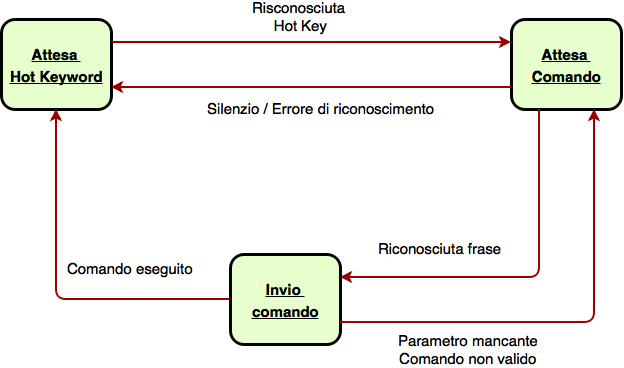
\includegraphics[width=\textwidth]{Conversation}
\caption{Diagramma di stato di una conversazione}
\label{fig:pose}
\end{figure}
\chapter{Voice}

Il software prevede un'interazione completamente vocale, si è perciò reso necessario comunicare con l'utente attraverso la voce.
L'utente riceve quindi un messaggio dopo aver inviato un comando, che lo informa a proposito della riuscita o a riguardo all'errore che è stato generato. Maggiori dettagli sono presenti nella sezione dedicata alla struttura della conversazione.
\section{Text To Speech}
Il modulo di text to speech è realizzato insieme al modulo di speech to text, anch'esso è quindi in python. Per semplicità si è delegato al sistema operativo il compito di effettuare lo speech to text. Nell'implementazione attuale è stato utilizzato il sistema operativo MAC OSX, quindi si è utilizzato il comando di sistema \textit{say}.

\section{Risposte}
Quando il software riceve un messaggio di risposta dopo l'esecuzione di un comando viene scelta casualmente una frase coerente con lo stato attuale del sistema.
Allo stato attuale non è presente un algoritmo di generazione automatica della frase che viene pronunciata.

\chapter{GUI}
\begin{figure}[H]
\centering
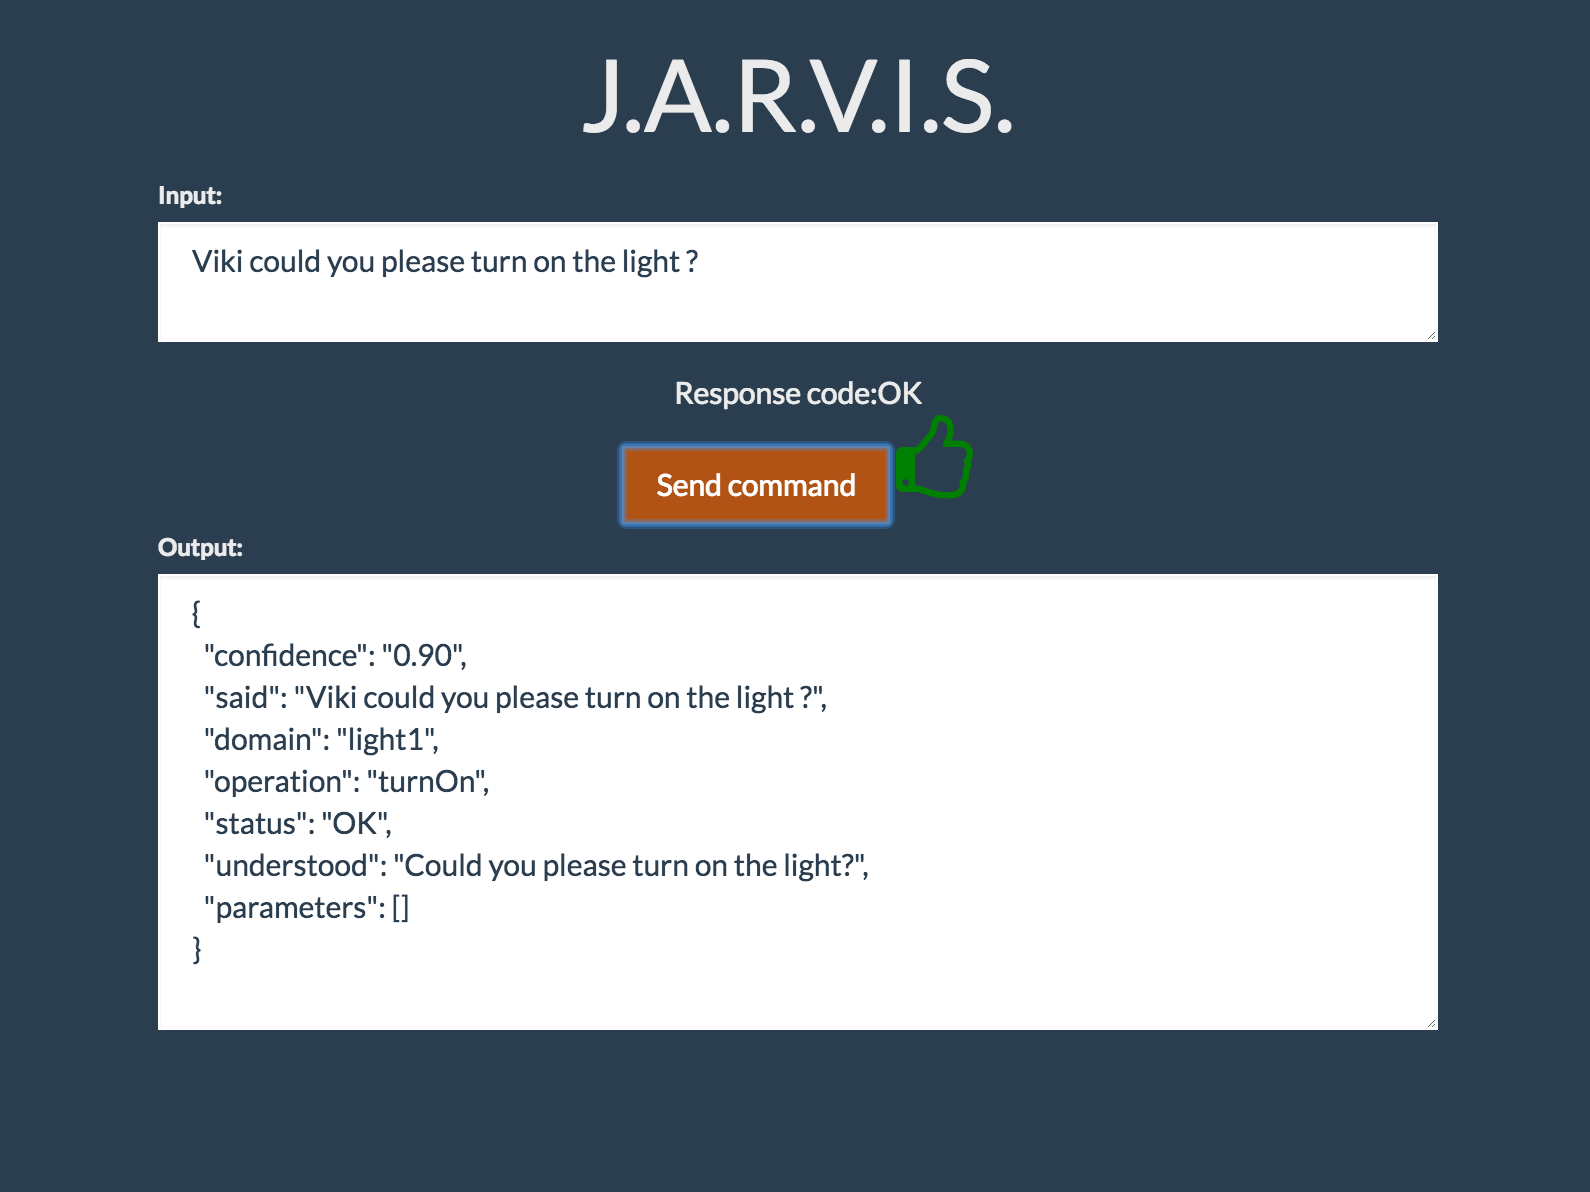
\includegraphics[width=\textwidth]{Gui}
\caption{Screen shut interfaccia gratica}
\label{fig:pose}
\end{figure}
Si è scelto di sviluppare un'interfaccia grafica che permettesse di interagire con il sistema senza passare dall'interazione vocale.

Essa si è resa necessaria per scopi di debug , ma può risultare utile utile quando non si può parlare o quando si vogliono avere maggiori informazioni a proposito di cosa sta accadendo nel sistema.
\section{Scelta tecnologica}
Inizialmente l'interfaccia grafica era stata realizzata in Java ed era integrata nel componente chiamato Brain; si è però ritenuto opportuno realizzare anch'essa come componente esterna al sistema.\\
Essendo esterna essa utilizza gli stessi canali di comunicazione utilizzati dall'interfaccia vocale, caratteristica utile nelle fasi di test della funzionalità del sistema.
Si è deciso di realizzare l'interfaccia grafica in Electron, il quale permette di creare finestre in maniera estremamente immediata; la semplice sintassi javascript ha permesso di sviluppare l'interfaccia in tempi molto brevi. \cite{electron}
\section{Electron}
Electron permette di realizzare delle applicazioni dekstop come se si stesse realizzando un sito web. Questo ha permesso la realizzazione di una semplice applicazione multi piattaforma scrivendo una sola volta il codice.
\section{Monitoraggio dei canali}
Visto che l' interfaccia grafica è realizzata come un componente esterno al sistema, i messaggi devono quindi essere inviati agli altri componenti del sistema attraverso i canali di comunicazione. Questo ha quindi permesso una maggior similarità tra l'interazione vocale e quella grafica, consentendo un debug del sistema più efficiente.
\section{Interfaccia}
Nella parte superiore della finestra è presente un campo di input dove viene inserito il comando che vuole essere eseguito. Al click del bottone send verrà inviato attraverso il canale socket.io al Brain.
Dopo l'invio del comando viene visualizzata nella parte centrale della finestra la risposta data dal sistema.
Nel caso in cui la risposta sia positiva viene visualizzata un'icona verde. Nel caso non sia stato possibile determinare un comando ne verrà visualizzata una rossa, infine nel caso manchi un parametro verrà visualizzata una gialla.

Nella parte bassa della finestra infine è presente un campo di testo dove vengono ricevuti i comandi dei quali Brain ha richiesto l'esecuzione.
\chapter{Elaborazione del comando}
Quando il sistema riceve un comando attraverso uno dei canali di input, viene inizializzata la pipeline di elaborazione del comando.

Questi sono i principali passaggi: 
\begin{itemize}
	\item Determinazione della distanza da domini
	\item Determinazione della distanza dalle operazioni
	\item Ricerca dei parametri
	\item Assegnazione dei parametri
	\item Calcolo dei valori di confidence
\end{itemize}
Nel caso il miglior comando abbia un valore di confidence sufficientemente alto esso viene eseguito. Se non fosse possibile allora vengono avviati i metodi alternativi di determinazione del comando :
\begin{itemize}
	\item Ricerca in memoria
	\item Ricerca di parametri per il comando precedente
\end{itemize}

\chapter{Ricerca Dominio e Operazione}
Dopo aver trasformato quanto detto dall'utente in testo, il sistema prova a mappare la frase su una delle azioni che che il sistema è in grado di eseguire.
In particolare viene cercato un dominio di esecuzione dell'operazione (es. Meteo, Luci) e l'operazione che si vuole compiere in questo dominio (es. Ricerca condizioni metereologiche, accensione della luce).


L'obbiettivo di questo sistema è di rendere generica l'interazione vocale, si è quindi dovuta trovare una metodologia che identificasse dominio e operazione indipendentemente dalle singole parole utilizzate, cercando quindi di astrarre il significato dai vocaboli.

 Il sistema per poter determinare l'operazione dispone di una lista di parole associate ad essa, una lista di parole associate al dominio e opzionalmente una lista di frasi per l'invocazione dell'operazione in un dominio specifico.

\section{Database lessicale : WordNet}
Il primo approccio si è basato sull'utilizzo di WordNet, un database lessicale della lingua inglese.
In WordNet ad ogni lemma è associata una definizione come in un normale dizionario, ma i lemmi sono anche collegati da una serie di relazioni, formando un grafo. In particolare le relazioni utilizzate nel progetto sono antonimia, iperonimia, sinonimia, metonimia.\cite{wordNet}

Utilizzando questo strumento è possibile reperire i sinonimi di una parola, dividendoli per categorie grammaticali (es. sinonimi di light come aggettivo o come nome).
Attraverso il confronto delle definizioni e delle relazioni è poi possibile determinare la similarità tra due vocaboli. Per definire tale metrica è possibile utilizzare diverse metodologie, tra le quali si è scelto di utilizzare quello definito come \textit{path}. \cite{wordNetWordSimilarity}

Questo approccio conta il numero di nodi che compongono il percorso più breve tra i due vocaboli, restituisce poi un coefficiente di similarità che corrisponde all'inverso della distanza precedentemente calcolata. Due vocaboli il cui significato è molto simile avranno delle strette relazioni con parole simili, quindi un alto coefficiente di similarità.\cite{wordNetPathSimilarity}
\subsection{Calcolo della similarità}
La similarità di un dominio con una frase viene calcolata come il massimo della similarità tra tutte le parole associate al dominio con tutte le parole presenti nella frase.

Lo stesso procedimento viene applicato alle operazioni .
\subsection{Vantaggi}
Vantaggi:
 \begin{itemize}
  \item \textbf{Richiede poche risorse}: il database pesa meno di 100Mb.
  \item \textbf{Supporto ai phrasal verbs}: sono già compresi nel database come un singolo verbo (es. turn\_off).
\end{itemize}
\subsection{Svantaggi}
\begin{itemize}
  \item \textbf{Dizionario statico}: è stato creato manualmente e non viene aggiornato da anni.  
  \item \textbf{Indipendente dalla frase}: il risultato dell'analisi di similarità è indipendente dall'ordine delle parole.
  \item \textbf{Dipendente dal POS}: per cercare i sinonimi solo nella corretta categoria grammaticale è necessario affidarsi al Part Of Speech tagger, la cui affidabilità non è totale.
\end{itemize}
\newpage
\section{Part-Of-Speech tagging}
L'approccio precedentemente descritto presenta lo svantaggio di non tenere conto dell'ordine delle parole nella frase; si è quindi pensato di aggiungere un componente che tenga in considerazione questa informazione.

Il Part Of Speech tagger è il componente che si occupa di assegnare a ogni parola un tag e di definire le relazioni che intercorrono tra questi .\cite{pos}\cite{posCategories}
\subsection{Calcolo della similarità}
La prima fase consiste nella ricerca di un nome che corrisponde al dominio, da essa vengono poi percorse delle relazioni che legano il verbo a colui che compie l'azione o colui che la subisce. Nei verbi viene quindi cercata l'azione con l'approccio di path similarity attraverso WordNet.
\subsection{Vantaggi}
\begin{itemize}
  \item \textbf{Dipendente dalla frase}: grazie alle relazioni tra le parole viene realmente tenuto conto del senso della frase, migliorando quindi l'affidabilità del sistema.
\end{itemize}
\subsection{Svantaggi}
\begin{itemize}
  \item \textbf{Eccessivamente dipendente dal POS}: l'analisi si basa completamente sui risultati del POS, sia per le relazioni che per i TAG, nel caso di errori di questo componente (il cui risultato non è sempre affidabile) l'intera analisi sarà corrotta.
\end{itemize}
I vari componenti POS (spaCy, ClearNLP, CoreNLP, MATE, Turbo, SyntaxNet) hanno un'affidabilità intorno al 93\%\cite{POS_scores}.

Questo tipo di analisi è estremamente difficoltoso nel caso di frasi la cui sintassi non è perfettamente corretta o eccessivamente gergale.  

Lo scopo del progetto è di rendere il più possibile flessibile il sistema: questo approccio avrebbe aumentato l'affidabilità al prezzo di rendere il sistema funzionante solo per frasi con una sintassi perfetta. Abbiamo quindi scelto di togliere questo componente dal sistema.
\newpage
\section{Doc2vec}
Gli approcci decritti fino ad ora si basano sulla linguistica.

Nel campo dell'NLP negli ultimi anni sono stati compiuti dei passi avanti, grazie ai miglioramenti nel machine learning. Approcci in questo ambito hanno raggiunto performance comparabili, se non migliori, del precedente stato dell'arte. 

La maggior parte degli algoritmi di machine learning richiede la trasformazione del testo in un vettore di dimensione fissa; generalmente l'approccio utilizzato è chiamato bag-of-words; esso però non tiene in considerazione l'ordine delle parole e la loro semantica.\cite{bow}

Doc2vec è un algoritmo che, come bag-of-words, permette di  rappresentare una parola, una frase, un paragrafo o un intero documento in un vettore di dimensione fissa. Risultati empirici hanno dimostrato che i vettori catturati attraverso Doc2vec sono significativi e riescono a condensare l'informazione di un testo di lunghezza variabile.\cite{doc2vec}
\subsection{Creazione del modello}
L'algoritmo precedentemente descritto per il suo funzionamento necessita di dati precedentemente classificati; se sul disco non è presente nessun modello, ne viene creato uno che associa le frasi associate alle operazioni (campo textInvocation del JSON di input) all'operazione stessa. 

Se è già presente un modello, queste frasi vengono aggiunte a quelle presenti. Dopo averlo completato viene avviata la fase di training dei vettori.
\subsection{Feedback}
Il sistema necessita di una grande mole di dati per l'allenamento dei vettori, si è quindi introdotto nel sistema di interazione vocale un metodo di feedback. Dopo l'esecuzione di un comando si ha la possibilità di notificare l'agente se il comando eseguito non è quanto si era richiesto, in caso contrario viene assunto che esso sia corretto. L'insieme delle frasi corrette viene quindi utilizzato successivamente per l'istruzione dei vettori.
\subsection{Calcolo della similarità}
Dopo aver istruito il modello e aver creato i vettori per ogni frase viene calcolato il vettore medio di tutte le frasi che rappresentano la stessa operazione. Quando l'utente pronuncia una frase viene calcolato l'angolo tra il vettore calcolato per la frase stessa e tutti i vettori medi precedentemente calcolati. Viene poi restituita all'utente la categoria associata al vettore più vicino
\begin{center}
\begin{math}
 \textit{similarity(A,B)} = \cos(\theta) = {A \cdot B \over \|A\| \|B\|}.
 \end{math}
 \end{center}
\subsection{Vantaggi}
\begin{itemize}
  \item \textbf{Dizionario dinamico}: il modello viene creato automaticamente e viene migliorato con il tempo.
  \item \textbf{Dipende dalla frase}: l'algoritmo considera l'ordine delle parole, cattura quindi la semantica della frase.
  \item \textbf{Miglioramento continuo}: il sistema è in grado di apprendere, migliora quindi con il tempo.
  \item \textbf{Indipendente dalle parole}: l'algoritmo di associazione del alle frasi lavora ad un livello di astrazione superiore alle parole, quindi non dipende da esse.
\end{itemize}
\subsection{Svantaggi}
\begin{itemize}
  \item \textbf{Grande mole di dati}: Per avere una classificazione accurata è necessario avere un grande numero di frasi associate a ogni operazione e ad ogni dominio
  \item \textbf{Piccole variazioni}: L'algoritmo fatica a percepire piccole variazioni che però modificano totalmente il senso della frase (turn on vs. turn off)
\end{itemize}
\subsection{Sviluppi futuri}
Si è empiricamente dimostrato che in una fase iniziale è difficile creare un modello sufficiente ad istruire il sistema. Non è quindi realizzabile un sistema che si basi solo su questo approccio nei tempi del progetto di bachelor. Si è comunque scelto di realizzare l'intera infrastruttura, così che con il passare del tempo il modella possa migliorare fino ad essere in grado di sostituire o almeno collaborare con l'infrastruttura attuale.
\newpage

%	Word2vec
\section{Word2vec}
I modelli precedentemente descritti possono essere racchiusi in due categorie:
\begin{itemize}
  \item \textbf{Statici}: WordNet, pos. Sono basati su un dizionario, non migliorano con il tempo.
  \item \textbf{Dinamici}: doc2vec, skip-thoughts vector(descritto in seguito). Sono basati su tecniche di deep learning, migliorano con il tempo, ma necessitano di un modello di allenamento.
\end{itemize}
Si è quindi cercato di ideare un approccio che riuscisse a eliminare la staticità derivante dall'utilizzo di un dizionario, senza però dover allenare direttamente una rete neurale.
Per fare ciò si è ideato sistema basato sull'algoritmo word2vec, il quale, attraverso una rete neurale a due livelli, prende come input del testo e restituisce una serie di vettori. 

Questo algoritmo è molto rapido nella sua fase di apprendimento, per questo motivo è possibile allenarlo su una grande base di dati (es. l'intero wikipedia), cosi che i vettori ottenuti siano generici.\cite{word2vec}
\subsection{Calcolo della correlazione}
 \[
 Sentence \quad\implies\quad "Switch\;on\;the\;lamp"
 \]
 \[
 S = 
\underbrace{["switch","on","the","lamp"]}_\text{n}
\]
 \[
 OperationsWords \quad\implies\quad "turnOn"
 \]
 \[
 O = 
\underbrace{["turn","on"]}_\text{m}
\]
 \[
 word similarity (a,b)= ws(a,b) = \arccos{{A \cdot B \over \|A\| \|B\|}}  
\]
 \[
 sentence\;distance = \frac{\sum_{i=1}^{m} min(ws(O_i \cdot s)\forall s \in S)} {m}
 \]
Per poter associare una frase pronunciata dall'utente ad un dominio e un'operazione viene sfruttata, come in doc2vec, la similarità del coseno. In particolare vengono confrontati i vettori rappresentanti le parole associate al dominio (array words del JSON) con tutte le parole nella frase, dopo di che viene ritornata la maggior correlazione trovata.

Lo stesso procedimento viene applicato alla ricerca dell'operazione. 

\subsection{Approccio ad albero}
Grazie a word2vec la similarità tra due parole viene ridotta a un prodotto scalare tra due vettori, il che è eseguito molto rapidamente. Il sistema calcola quindi il valore si similarità di tutti i domini, poi calcola la similarità di tutte le operazioni associate a tutti i domini e non solo il migliore. 
\subsection{Vantaggi}
\begin{itemize}
  \item \textbf{Dizionario dinamico}: il modello viene creato automaticamente, può essere addestrato su qualunque base di dati.
  \item \textbf{Efficiente}: l'intero calcolo della similarità è ricondotto a prodotti scalari.
    \item \textbf{Indipendente dalle parole}: l'algoritmo apprende, quindi riesce ad imparare nuove parole.
\end{itemize}
\subsection{Svantaggi}
\begin{itemize}
  \item \textbf{Scelta del modello}: le prestazioni e le risorse utilizzate dipendono dalla scelta del modello. Maggiori informazioni nel capitolo dedicato.
  \item \textbf{Parole composte}: con le classiche tecniche di allenamento i vettori vengono create per singole parole, non sono quindi supportati dal sistema i phrasal verbs.
\end{itemize}
\subsection{Parole composte}
Nel caso in cui a un'operazione o a un dominio si voglia associare una parola composta, ad esempio "turn off", essa deve essere aggiunta al vettore delle parole associate seguendo la convenzione dei nomi "Lower Camel Case". Il calcolo della similarità verrà poi effettuato come la media della similarità dei token che compongono la parola.\cite{lcc}
\subsection{Phrasal verbs}
Come evidenziato negli svantaggi il sistema non sarebbe in grado di analizzare la similarità una una parola composta, ad esempio "turn on", e una parola singola che possiede lo stesso significato, ad esempio "activate".
Per questo motivo, in fase di caricamento del sistema, quando vengono analizzate le parole associate a ogni operazione o dominio, un modulo dedicato si occupa di aggiungere automaticamente sinonimi della parola.

Nella maggior parte dei casi nei sinonimi è contenuto un verbo della categoria opposta (un phrasal verb per un verbo composto da una parola singola e l'inverso).
Il problema potrebbe essere risolto con un modello word2vec che contiene phrasal verbs e parole composte.

\chapter{Ricerca dei parametri}
Come descritto nei capitoli precedenti, ai comandi possono essere assegnati dei parametri che appartengono a determinati tipi, definiti da ParameterType.

Per ogni tipologia di parametro si è creata una struttura capace di trovare valori della specifica tipologia di parametro in una frase.
\section{Assegnazione dei parametri}
Il software si occupa di ricercare i parametri di ogni tipologia possibile, dopo aver determinato i valori assunti dai parametri essi vengono assegnati ai comandi. 
\section{Ricerca dei migliori parametri}
In una prima implementazione del sistema venivano cercati i parametri solo dei comandi che venivano ritenuti più probabili dopo l'analisi di attinenza ai domini e alle operazioni.\\
 Questo approccio permetteva di effettuare la ricerca solo per un numero ristretto di comandi, ma trascurava l'informazione relativa ai parametri trovati nella frase nel calcolo della confidence. 

Dall'analisi dei risultati risultati è emerso come il numero di informazioni considerate per il calcolo della confidence non fosse sufficiente.
\section{Ricerca di tutti i parametri}
Per migliorare l'affidabilità nel sistema si è scelto di utilizzare l'informazione relativa ai parametri trovati nella frase per il calcolo della confidence. \\Intuitivamente se una frase contiene un Colore è più probabile che sia relativa a un comando che ha come parametro un colore ed è meno probabile che sia relativa a un comando che non può prendere come parametro un colore.\\
\subsection{Aumento confidenza comando}
Quando viene trovato un parametro appartenente a una determinata tipologia esso viene assegnato a tutti i comandi che possiedono quel tipo di parametro. L'assegnazione provoca un aumento della percentuale che quel comando sia uno dei comandi più coerenti con la frase sentita. Il peso di questo aumento verrà calcolato solo successivamente.
\section{Color}
\begin{center}
\[
I\;want\;my\;light\;to\;turn\;
\underbrace{red}
\quad\implies\quad Color = [255,0,0]
\]
\[
Set\;light\;color\;to\;
\underbrace{dark\;slate\;blue}
\quad\implies\quad Color = [72,61,139]
\]
\end{center}

Il sistema è in grado di ricercare i colori secondo la nomenclatura X11; essa associa a ogni nome di colore i suoi valori nei formati : RGB, HSL/HSV, HSL, HSV. Si è optato per l'utilizzo del formato RGB, che viene rappresentato come un vettore composto da 3 elementi di tipo intero.\cite{x11Colors}

La ricerca del colore nella frase viene effettuata tramite un' espressione regolare. Nel caso nella frase compaia un colore composto da più parole, viene preferito il colore con un maggior dettaglio.
Per esempio "I want my lamp to turn light blue" restituirà il colore "Light blue" e non "Blue".
\section{Number}
\[
Set\;the\;volume\;level\;to\;
\underbrace{75.5}
\quad\implies\quad Number = +75.5
\]
Il sistema è in grado di riconoscere numeri, espressi attraverso cifre. Questo è possibile in quanto i sistemi di Speech to Text utilizzati traducono i numeri espressi attraverso parole in cifre.

I numeri possono rappresentare delle percentuali, avere cifre decimali (usando come separatore '.') e un segno di positività o negatività. La ricerca viene effettuata attraverso un'espressione regolare.
\section{Location}
\[
What's\;the\;weather\;like\;on\;the\;
\underbrace{Alps}
\quad\implies\quad Location = Alps
\]
\[
How'\;s\;the\;weather\;in\;
\underbrace{London}\;?
\quad\implies\quad Location = London
\]
Il sistema è in grado di riconoscere nella frase le parole che rappresentano un luogo.
I luoghi vengono rappresentati direttamente attraverso il loro nome, in quanto diverse API (es. yahoo meteo e google meteo) permette di sottomettere richieste direttamente in questo formato.

Il riconoscimento viene effettuato sfruttando il componente di CRF Named Entity Recognizer, parte del pacchetto StanfordNLP. \cite{stanfordNer}
\subsection{Stanford Named Entity Recognizer}
Stanford NER è un'implementazione Java di un software in grado di assegnare delle etichette a sequenze di parole, che rappresentano persone, organizzazioni e luoghi.
Il software viene offerto insieme con il un modello allenato per l'inglese, utilizzato nella nostra implementazione, ma potrebbe essere allenato con altri dati nel caso fosse necessario ad esempio cambiare lingua.
\section{Date Time}
\begin{center}
\[
Remind\;me\;that\;\;
\underbrace{the\;day\;after\;tomorrow}
\quad\implies\quad DateTime = 2016-08-14
\]
\[
Wake\;me\;up\;\;
\underbrace{at\;9\;am,\;tomorrow\;morning}
\quad\implies\quad DateTime = 2016-08-20T09:00
\]
\[
Turn\;on\;the\;light\;
\underbrace{every\;15\;minutes}
\quad\implies\quad DateTime = T15MX
\]
\end{center}
Il sistema è in grado di riconoscere orari, date, espressioni temporali, eventi periodici. La ricerca dei valori di tipo DateTime viene effettuata attraverso il componente SUTime, compreso nella suite StanfordNLP.\cite{stanfordSUTime}

\subsection{Stanford SUTime}
E' un componente che fa parte della suite di natural language processing di Stanford; esso è basato su un sistema di regole, il suo output è quindi deterministico.

Le regole utilizzate da questo componente sono disponibili solo per la lingua inglese, è quindi uno dei pochi componenti del nostro sistema che impone l'utilizzo della lingua inglese per l'intero sistema.

\newpage
\section{Parametri nella frase sucessiva}
Nel caso il sistema dovesse riconoscere un comando per il quale è mancante un parametro, esso è in grado di ricercare il valore assunto del parametro nella frase successiva.
\subsection{Esempio conversazione}
\begin{dialogue}
\speak{Utente} Viki, Set the light intensity.
\speak{Sistema} A number is missing!
\speak{Utente} I would like 80\%.
\speak{Sistema} Done.
\end{dialogue}



\chapter{Determinazione miglior comando}
Il valore di confidenza che viene assegnato ad un comando viene assegnato in 3 differenti fasi:
\begin{itemize}
  \item \textbf{Dominio}: Corrisponde alla distanza minima tra le parole associate al domino e quelle presenti nella frase.
  \item \textbf{Operazione}: Corrisponde alla distanza minima tra le parole associate all'operazione e quelle presenti nella frase.
  \item \textbf{Parametri}: Valore positivo nel caso siano stati trovati parametri assegnabili al comando, valori negativi se sono stati trovati parametri non assegnabili al comando.
\end{itemize}
Dati questi tre parametri è necessario decidere quale comando è più probabile che sia quello indicato nella frase; inoltre è necessario determinare se il comando più probabile deve essere realmente eseguito o se la sua aderenza a quanto pronunciato dall'utente non è sufficiente.
\begin{center}
\[
\boldsymbol{D_{d}} = Distanza\;tra\;dominio\;e\;frase\;pronunciata
\]
\[
\boldsymbol{D_{o}} = Distanza\;tra\;operazione\;e\;frase\;pronunciata
\]
\[
\boldsymbol{P_{t}} = Numero\;di\;parametri\;assegnabili\;al\;comando
\]
\[
\boldsymbol{C} = Confidenza\;attribuita\;al\;comando
\]
\[
\boldsymbol{C} = f(D_{d} ,D_{o},P_{t})
\]
\end{center}
\newpage
\section{Esempio}
\[
Set\;the\;light\;intensity\;to\;
\underbrace{22}
\quad\implies\quad Number = 22
\]
\begin{figure}[H]
\centering
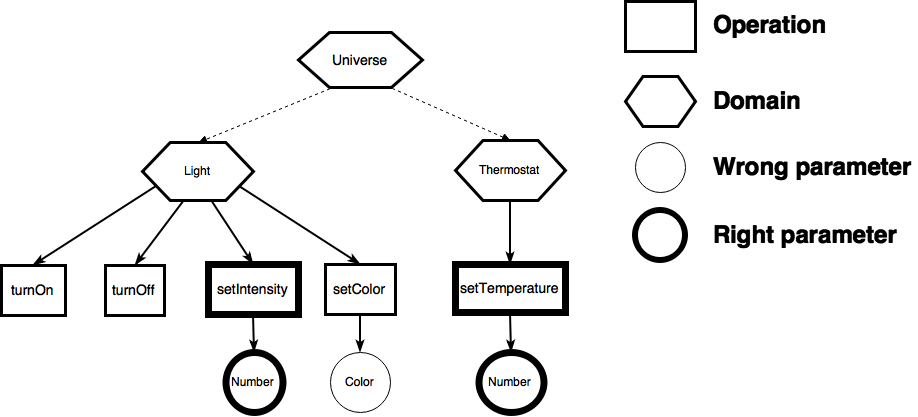
\includegraphics[width=\textwidth]{Confidence}
\caption{Albero di determinazione della confidence}
\label{fig:pose}
\end{figure}
Nella frase soprastante il sistema di ricerca dei parametri ha trovato un numero.\\
I comandi che implicano la presenza di un numero, setIntensity e setTemperature, ricevono un bonus.\\
Il comando setColor, che possiede un parametro di tipo Colore viene invece penalizzato, in quanto non è coerente con il numero trovato nella frase.
\section{Funzioni statiche}
Per poter definire il valore di confidenza da assegnare ad ogni comando si è reso necessario creare una funzione che tenga in considerazione distanza dal domino, dall'operazione e il contributo dei parametri.
Inizialmente si è optato per la definizione di una funzione che potesse rispettare l'importanza delle varie componenti.
La funzione, definita in maniera intuitiva, è la seguente :
\[
\boldsymbol{C} = f(D_{d} ,D_{o},P_{t}) = 0.5*D_{d}+0.5*D_{o}+0.3*P_{t}
\]
Essa tiene in considerazione ugualmente il contributo fornito dal domino e quello dell'operazione. Infine garantisce un bonus ai comandi ai quali è stato assegnato un parametro e un malus ai comandi che non possiedono i parametri delle tipologie trovate nella frase.
\subsection{Vantaggi}
\begin{itemize}
  \item \textbf{Veloce}: La funzione è un semplice calcolo, non richiede quindi operazioni computazionalmente complesse.
   \item \textbf{Facilmente gestibile}: Non basandosi su tecniche di machine learning lo sviluppatore può modificare direttamente la funzione.
  \item \textbf{No Data set}: Non richiede l'utilizzo di un dataset per fare il training del sistema.
\end{itemize}
Per questi motivi questa versione è stata utilizzata durante le fasi di sviluppo del sistema.
\subsection{Svantaggi}
\begin{itemize}
  \item \textbf{Statica}: Non migliora con il passare del tempo.
   \item \textbf{Difficile da generalizzare}: Sarebbe molto complesso riuscire a definire manualmente una funzione che dia un risultato corretto con tutte le combinazioni di parametri.
\end{itemize}

\section{Machine learning}
L'approccio esposto nella sezione precedente conferisce troppa staticità al sistema, si è quindi optato per una metodologia di determinazione della confidenza assegnata a un comando basata su tecniche di machine learning.

Tra i vari approcci disponibili si è scelto di utilizzare naive Bayes, per la sua rapidità di calcolo. E' infatti necessario calcolare il valore di confidenza per ognuno dei possibili comandi che potrebbe essere eseguito; il cui numero potenzialmente potrebbe essere molto elevato.
\subsection{Naive Bayes classifier}
L'algoritmo di naive Bayes viene utilizzato per la classificazione, assumendo che le caratteristiche osservate siano indipendenti tra loro, la classificazione viene effettuata attraverso il teorema di Bayes.

$$ P(A \mid B) = \frac{P(B \mid A) \, P(A)}{P(B)} $$

Questa assunzione può essere fatta anche se gli eventi non sono perfettamente indipendenti, è infatti stato dimostrato che le performance sono comunque buone. Questo algoritmo è caratterizzato dalla velocità; la probabilità viene infatti calcolata in maniera diretta attraverso delle operazioni aritmetiche.

Grazie a quest'algoritmo è possibile calcolare la possibilità di appartenenza a una classe, date le caratteristiche dell'oggetto.

\subsection{Discretizzazione}
Naive Bayes richiede che le feature siano discrete; per il funzionamento del sistema è inoltre importante che il numero di categorie sia il minore possibile, non è quindi possibile utilizzare direttamente il valore di distanza utilizzato fino ad ora nel sistema, che è salvato il un valore di tipo \textit{double}.

Per ovviare questo problema sono state create creare 10 categorie di distanza, segmentando a tratti di 0.1 il valore precedentemente calcolato.
\subsection{Vantaggi}
\begin{itemize}
  \item \textbf{Veloce}: Il tempo di calcolo di naive Bayes è costante.
  \item \textbf{Dinamico}: Il sistema impara con il tempo, continua a migliorare e riesce a gestire la situazione limite.
\end{itemize}
Data la dinamicità e le migliori performance del sistema si è scelto di utilizzare questo sistema nell'implementazione finale.
\subsection{Svantaggi}
\begin{itemize}
  \item \textbf{Minor controllo}: Non si può modificare direttamente la funzione di calcolo della confidence.
  \item \textbf{DataSet}: Per il corretto funzionamento del sistema è necessario definire un dataset, che serve durante la fase di training e di verifica.
\end{itemize}
\chapter{Algoritmo di apprendimento}
L'approccio utilizzato per associare i comandi alla frasi pronunciati dall'utente è basato sulla similarità delle parole, ci sono però alcuni casi nei quali alcune espressioni con lo stesso significato utilizzano vocaboli molto differenti tra loro.

Per poter far comprendere queste casistiche al sistema sarebbe stato necessario rivoluzionare l'algoritmo, si è quindi optato per aggiungere una funzione al sistema che permettesse di insegnare comandi arbitrari al sistema.

L'aggiunta di questo algoritmo permette quindi all'utente finale di poterlo programmare, interagendo direttamente con la voce. Questo rende possibile la creazione di comandi rapidi per l'esecuzione di operazioni comuni ed è possibile insegnare al sistema espressioni gergali.
\section{Comando di apprendimento}
Per poter insegnare un comando al sistema è necessario che l'ultima frase sottoposta sia stata classificata come sconosciuta. 

Il riconoscimento del comando di apprendimento viene eseguito esattamente come avviene per gli altri comandi, infatti durante la fase di caricamento dell'universo viene iniettato un comando fittizio che serve per apprendere. Questo garantisce flessibilità al sistema, che anche in questa circostanza non è legato a una frase specifica.

Dopo che il sistema si è dichiarato pronto ad apprendere esso rimane in attesa di una frase dalla quale è in grado di determinare un comando, può quindi essere un ricordo già presente o direttamente un comando.

Dopo la conferma di avvenuto apprendimento il sistema sarà in grado di riconoscere il nuovo comando e cercherà di generalizzarlo per riconoscere comandi simili ad esso.
\section{Generalizzazione del comando}
La memoria dei sistema è costituita da una mappa composta di coppie frase-comando. Il sistema però non è solo in grado di riconoscere esattamente la frase presente nel ricordo.
Durante la fase di ricerca nella memoria il sistema si occupa di confrontare la frase pronunciata dall'utente con quelle presenti nel ricordo, se uno dei ricordi non è identico a quanto pronunciato, ma è sufficientemente simile, il comando viene restituito.
\subsection{Similarità di frasi}
Per confrontare i ricordi legati alle frasi si è ideato un semplice algoritmo che permette di calcolare la similarità tra frasi. Esso sfrutta lo stesso modello \textit{word2vec} usato nella ricerca di domini e operazioni.

Il coefficiente di similarità è costituito dalla media aritmetica della distanza minima tra le parole che compongono la frase e le parole che compongono il ricordo.

\subsection{Esempio conversazione}
\begin{dialogue}
\speak{Utente} Viki, Goodnight.
\speak{Sistema} I'm sorry, i do not know what does it mean
\speak{Utente} Let me teach you something
\speak{Sistema} Ok, I'm ready to learn.
\speak{Utente} Turn off the light.
\speak{Sistema} Learned.
\end{dialogue}
\begin{dialogue}
\speak{Utente} Viki, Goodnight.
\speak{Sistema} Done.
\end{dialogue}

\section{Persistenza della memoria}
La struttura che rappresenta la memoria è costituita da un oggetto Java, per questo motivo la persistenza è stata realizzata attraverso la serializzazione.

Durante la fase di spegnimento del sistema la memoria viene persistita su file, all'avvio del sistema viene controllato se è presente un file rappresentante la memoria e nel caso sia presente viene utilizzato come memoria attuale.

\chapter{Configurazione}
I vari moduli realizzati necessitano di diverse configurazioni per poter funzionare correttamente. Si è quindi ritenuto opportuno esporre tutti i parametri in un file di proprietà che viene letto durante l'avvio dei vari sistemi. 

Così facendo è possibile cambiare gli indirizzi i rete, i valori dei canali di comunicazione e i percorsi per i file senza dover modificare il codice sorgente.

Nel caso alcuni parametri fossero mancanti o considerati errati sono presenti dei valori di default.
Le proprietà configurabili sono :
\begin{itemize}

  \item \textbf{WordNet dictionary path}: Percorso del file del database di WordNet.
   \item \textbf{Color dictionary path}: Percorso del file del file di dizionario dei colori.
      \item \textbf{Viki universe path}: Percorso del file da utilizzare come universo, nel caso si voglia caricare da file.
      \item \textbf{Log path}: Percorso del file da utilizzare come log file.
      \item \textbf{Memory path}: Percorso del file da utilizzare come memoria.
      \item \textbf{Viki get URL}: Indirizzo della chiamata che espone la rappresentazione dell'universo.
      \item \textbf{Command receiver address}: Indirizzo al quale avviare il server socket.io
      \item \textbf{Command receiver port}: Port al quale avviare il server socket.io
      \item \textbf{Text command message}: Namespace dei comandi socket.io da ricevere.
      \item \textbf{Viki address }: Indirizzo al quale inviare i comandi da eseguire.
      \item \textbf{Command message }: Namespace dei comandi socket.io da inviare.
      \item \textbf{Min confidence }: Valore di confidenza sotto al quale un comando non è considerato valido.
      \item \textbf{Learning rate}: Valore sopra il quale due frasi vengono considerate equivalenti.
\end{itemize}

\chapter{Risultati}
Per poter analizzare le performance del sistema si è creato un moke up di una casa, comprendente 10 domini, per un totale di 31 operazioni. \\
Successivamente sono state raccolte 80 frasi che l'utente avrebbe pronunciato alla casa per interagire con le varie funzionalità.
\section{Svolgimento dei test}
Per valutare la risposta del sistema si è creato un ambiente di test, che riceve in input le frasi pronunciate dall'utente e gli identificativi di dominio e operazione al quale essa si riferisce.\\
Ogni frase viene sottoposta al sistema, il quale ricava il comando associato, che viene poi confrontato con gli id ricevuti.\\
Ogni output viene poi classificato tra comandi corretti, sbagliato o frasi al quale al sistema non è riuscito ad associare un comando.
\section{Analisi dei risultati}
L'algoritmo sviluppato si è dimostrato in grado di riconoscere correttamente frasi nelle quali vengono utilizzate parole che non erano state associate ai metodi in configurazione, è stato inoltre in grado di riconoscere comandi indipendentemente dalla sintassi della frase.\\
Esso ha riconosciuto con successo 58 comandi su 80 (72,5\%).
\subsection{Limiti riscontrati}
I componenti che si occupano dell'associazione di frasi a comando non è vincolato da un sistema di grammatiche, ma si sviluppa principalmente in due diversi stati : associazione al dominio e all'operazione, per questo motivo riesce a riconoscere prevalentemente frasi che possiedono riferimenti sia all'operazione, sia al domino. \\
Per questo motivo frasi nelle quali una sola parola rappresenta sia il dominio, che l'operazione o frasi nelle quali uno dei sue elementi dovrebbe essere dedotto dal contesto, non sono sempre riconosciute.
\[
 Make\;it
\underbrace{louder\;}_\text{Domain\;and\;Operation}
 \quad\implies\quad Non\;riconosciuto
\]
\[
 Could\;you\;please\;
\underbrace{increase\;}_\text{Operation}the
\underbrace{\;volume?}_\text{Domain}
 \quad\implies\quad Risconosciuto
\]
\section{Istruire il sistema}
La maggior parte dei comandi che non sono stati riconosciuti dal sistema sono espressioni gergali o sfruttano informazioni deducibili dal contesto, queste espressioni potrebbero essere insegnate al sistema attraverso l'algoritmo di apprendimento. \\
Grazie a questa alternativa la percentualmente di successo del sistema può crescere costantemente, fino ad arrivare alla comprensione della quasi totalità dei comandi.
% Modelli
\chapter{Modelli word2vec}
Il sistema descritto nella sezione precedente basa il calcolo della similarità sui vettori estratti dal modello. Essi sono direttamente correlati al corpus \cite{corpus} utilizzato per l'istruzione della rete neurale. Nel web sono presenti modelli già allenati su basi di dati di grandi dimensioni \cite{trained_models}.

Data la dimensione di del corpus sono presenti un insieme di parole che è molto superiore a quelle che possono essere utilizzate all'interno di un ambiente di automazione casalinga. Sempre grazie alla mole di dati però questi vettori rappresentano pienamente il senso di una parola, al punto di essere utilizzabili in numerosi contesti.
\section{Google word2vec}
Nella prima implementazione del sistema si è scelto di utilizzare il modello fornito insieme all'implementazione di google, il quale è stato addestrato sull'intero google news. I suoi vettori possiedono 300 dimensioni e rappresentano 3 milioni di parole. Questo modello è molto generico, ma le sue dimensioni sono elevate, infatti il sistema necessità di circa 8GB di memoria RAM per il suo funzionamento.
\section{Allenamento di un Modello}
Per migliorare le performance del sistema si potrebbe sostituire il modello fornito da google con un modello addestrato su parole e frasi che realmente possono essere di interesse all'interno di un ambiente domestico. Per questo motivo il lo stesso sistema di logging delle frasi utilizzato da doc2vec viene utilizzato per istruire un modello proprietario. Nei tempi del progetto di bachelor si ritiene che non sia possibile raggiungere la massa di informazioni necessaria a creare dei vettori che riescano a catturare il significato delle parole. Esso potrebbe essere uno sviluppo futuro del sistema, dopo qualche mese di utilizzo quotidiano. L'implementazione realizzata contiene le funzioni necessarie all'istruzione di un modello ed è predisposta a sostituire il modello attuale.
\section{sense2vec}
I modelli allenati con word2vec associano a ogni parola un vettore, anche quando questa parola assume più significati, il vettore tende poi verso il significato più comune. Per ovviate questo problema è nato sense2vec, il quale associa a ogni parola più vettori, uno per ogni significato. É possibile ad esempio creare il vettore corrispondente a una parola associata al suo Part Of Speech Tag.  \cite{posCategories} \cite{sense2vec} 

Con lo stesso approccio è anche possibile unire in un vettore più parole, ad esempio i phrasal verbs, cosi da poter mappare un senso e non una sola parola in un vettore. Si è quindi pensato che, una volta raggiunta la necessaria quantità di informazioni, si potrebbe creare un modello seguendo questo approccio, cosi da eliminare il dizionario WordNet dal sistema.

\chapter{Sviluppi futuri}
Il progetto sviluppato aspira a creare un'interfaccia naturale per una casa intelligente, dato il breve periodo a disposizione non è stato possibile realizzare tutte le funzionalità ideate, si elencano nelle sezioni seguenti i possibili sviluppi futuri del sistema.
\section{Incremento vincoli}
In ogni sistema che si occupa di effettuare riconoscimento vengono imposti dei vincoli, l'incremento della sensitività provoca un aumento dei falsi negativi e una diminuzione dei falsi positivi.
Nell'implementazione si è cercato di rimuovere molti vincoli, diminuendo notevolmente i falsi negativi, incrementando però i falsi positivi.
Si potrebbero quindi migliorare il sistema aumentandone i vincoli.
\begin{figure}[H]
\centering
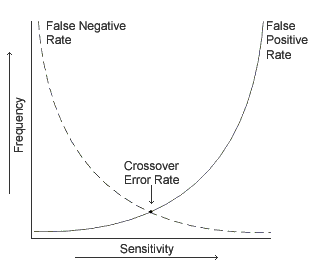
\includegraphics[scale=0.8]{falseRate}
\caption{Diagramma falsi positivi e falsi negativi}
\label{fig:pose}
\end{figure}
\subsection{Sentence similarity}
Nel sistema per calcolare la distanza tra un dominio o un operazione e una frase vengono confrontati i vettori relativi alle parole. Si potrebbe migliorare il sistema unendo l'informazione derivante dal POS, confrontando il vettore relativo alla parola collocata nella categoria grammaticale.

Una modifica di questo tipo permetterebbe di distinguere ad esempio la parola "light" usata come nome, rispetto a "light" usata come verbo.
\subsection{Ricerca avanzata dei parametri}
Nell'implementazione attuale i parametri vengono cercati nella frase in modo arbitrario, un' implementazione più raffinata potrebbe cercare il parametro solo nei complementi del verbo. Questo potrebbe però a un notevole incremento della richiesta in termini di capacità di calcolo, in quanto la ricerca dei parametri andrebbe effettuata per ogni comando.

\section{Comandi condizionali}
Il sistema è ora in grado di chiedere informazioni e di eseguire comandi, si potrebbe quindi creare un sistema di regole in grado di effettuare alcuni comandi in concomitanza con l'esecuzione di degli eventi.
Dopo aver preparato il sistema per la gestione dei comandi condizionali sarebbe necessario predisporre l'interfaccia in linguaggio naturale per riconoscere questa tipologia di comandi.

Si dovrebbe ideare un modulo in grado di comprendere la condizione da assegnare al comando e andrebbe esteso il formalismo di trasmissione dei comandi attuale, per permettere la trasmissione della condizione.

Il sistema di regole utilizzato potrebbe inoltre essere compatibile con il servizio IFTTT.\cite{ifttt}
\section{MultiLingua}
L'interfaccia naturale del sistema sviluppata in questo progetto è stata ideata per la lingua inglese. Si è però cercato di limite al minimo i vincoli alla lingua, di seguito un elenco dei vari componenti e eventuali limitazioni a proposito della lingua:
\begin{itemize}
      \item \textbf{Hot keyword detector}: Il componente è indipendente dalla lingua.
      \item \textbf{Sentence listener}: Il componente è indipendente dalla lingua, richiede però che essa venga specificata a priori.
      \item \textbf{DomainOperation finder}: Il componente è indipendente dalla lingua, richiede però che venga allenato un modello di word2vec specifico per la lingua che si vuole utilizzare.
      \item \textbf{Number finder}: Il componente è indipendente dalla lingua.
      \item \textbf{Color finder}: Il componente si basa su un database dei colori in lingua inglese, sarebbe però sufficiente sostituire il file.
      \item \textbf{DateTime finder}: Il componente offerto da Stanford è stato ideato per la lingua inglese, bisognerebbe quindi creare un nuovo componente.
\end{itemize}
Il sistema è quindi per la maggior parte predisposto per cambiare la lingua utilizzata, per estenderlo a una nuova lingua l'unico sforzo consistente sarebbe quindi costituito dalla creazione di un nuovo componente in grado di trovare i valori dei parametri di tipo DateTime.
\chapter{Conclusione}
Il progetto di tesi si pone come obiettivo principale la realizzazione di un infrastruttura che migliori la qualità dell'interazione vocale tra l'utente e l'ambiente domotico.\\
L'architettura realizzata ha dimostrato come sia possibile realizzare un'agente in grado comprendere comandi in modalità di ascolto always-on e che provveda alla loro interpretazione senza che siano presenti vincoli ai quali l'utente si deve attenere.\\
Quanto realizzato è in grado di apprendere dall'utente nuovi modi di interagire con il comando, il quale può quindi addestrare il sistema per farlo aderire alle sue esigenze e migliorarne le performance.\\
La flessibilità del sistema riesce a garantire una conversazione più naturale rispetto al prodotto precedente.\\
L’assenza di regole fisse solleva l’utente dal dover pensare a come trasmettere il comando al sistema, in quanto può comportarsi come durante una normale conversazione; questo permette quindi anche gli utenti meno esperti di usufruire del sistema.\\

\bibliographystyle{unsrt}
\bibliography{bibliografia}
\begin{appendices}
\chapter{Home moke-up}
\begin{lstlisting}[language=json,firstnumber=1]
{
    "domains": [
        {
            "id": "light1",
            "words": [
                "lamp",
                "light"
            ],
            "friendlyNames": [
                "sphere",
                "ball"
            ],
            "operations": [
                {
                    "id": "turnOff",
                    "textInvocation": [
                        "Could you please turn off the light?"
                    ],
                    "words": [
                        "turnOff"
                    ]
                },
                {
                    "id": "turnOn",
                    "textInvocation": [
                        "Could you please turn on the light?"
                    ],
                    "words": [
                        "turnOn"
                    ]
                },
                {
                    "id": "isOn",
                    "textInvocation": [
                        "Is the light on?"
                    ],
                    "words": [
                        "isOn"
                    ]
                },
                {
                    "id": "isOff",
                    "textInvocation": [
                        "Is the light off?"
                    ],
                    "words": [
                        "isOff"
                    ]
                },
                {
                    "id": "setIntensity",
                    "textInvocation": [
                        "Set light intensity to 80%"
                    ],
                    "mandatoryParameters": [
                        {
                            "id": "intensity",
                            "type": "NUMBER"
                        }
                    ],
                    "words": [
                        "setIntensity"
                    ]
                },
                {
                    "id": "setColor",
                    "textInvocation": [
                        "Set light color to red"
                    ],
                    "mandatoryParameters": [
                        {
                            "id": "color",
                            "type": "COLOR"
                        }
                    ],
                    "words": [
                        "setColor"
                    ]
                },
                {
                    "id": "getColor",
                    "textInvocation": [
                        "Which color is the lamp"
                    ],
                    "words": [
                        "getColor"
                    ]
                }
            ]
        },
        {
            "id": "heater1",
            "words": [
                "heater",
                "thermostat"
            ],
            "operations": [
                {
                    "id": "turnOn",
                    "textInvocation": [
                        "Turn on the heater"
                    ],
                    "words": [
                        "turnOn"
                    ]
                },
                {
                    "id": "turnOff",
                    "textInvocation": [
                        "Turn off the heater"
                    ],
                    "words": [
                        "turnOff"
                    ]
                },
                {
                    "id": "getTemperature",
                    "textInvocation": [
                        "What's the temperature?"
                    ],
                    "words": [
                        "getTemperature"
                    ]
                },
                {
                    "id": "setTemperature",
                    "textInvocation": [
                        "Set the heater temperature to 21"
                    ],
                    "mandatoryParameters": [
                        {
                            "id": "temperature",
                            "type": "NUMBER"
                        }
                    ],
                    "words": [
                        "setTemperature"
                    ]
                },
                {
                    "id": "increaseTemperature",
                    "words": [
                        "increaseTemperature","turnUpTemperature"
                    ]
                },
                {
                    "id": "decreaseTemperature",
                    "words": [
                        "decreaseTemperature","turnDownTemperature"
                    ]
                }
            ]
        },
        {
            "id": "weather",
            "words": [
                "weather"
            ],
            "operations": [
                {
                    "id": "getWeather",
                    "textInvocation": [
                        "What's the weather in London?"
                    ],
                    "optionalParameters": [
                        {
                            "id": "location",
                            "type": "LOCATION"
                        },
                        {
                            "id": "date",
                            "type": "DATETIME"
                        }
                    ],
                    "words": [
                        "get",
                        "what",
                        "is"
                    ]
                }
            ]
        },
        {
            "id": "telephone",
            "words": [
                "telephone"
            ],
            "operations": [
                {
                    "id": "pickUp",
                    "words": [
                        "pickUp",
                        "answer"
                    ]
                },
                {
                    "id": "hangUp",
                    "words": [
                        "hangUp","end"
                    ]
                }
            ]
        },
        {
            "id": "timer",
            "words": [
                "timer"
            ],
            "operations": [
                {
                    "id": "remind",
                    "words": [
                        "remind"
                    ],
                    "mandatoryParameters": [
                        {
                            "id": "when",
                            "type": "DATETIME"
                        },
                        {
                            "id": "what",
                            "type": "FREE_TEXT"
                        }
                    ]
                }
            ]
        },
        {
            "id": "alarm",
            "words": [
                "alarm"
            ],
            "operations": [
                {
                    "id": "turnOn",
                    "words": [
                        "turnOn",
                        "activate"
                    ]
                },
                {
                    "id": "turnOff",
                    "words": [
                        "turnOff",
                        "deactivate"
                    ]
                }
            ]
        },
        {
            "id": "lights",
            "words": [
                "lamps",
                "lights",
                "everyLight",
                "allLamps"
            ],
            "operations": [
                {
                    "id": "turnOff",
                    "textInvocation": [
                        "Could you please turn off the light?"
                    ],
                    "words": [
                        "turnOff"
                    ]
                },
                {
                    "id": "turnOn",
                    "textInvocation": [
                        "Could you please turn on the light?"
                    ],
                    "words": [
                        "turnOn"
                    ]
                },
                {
                    "id": "setIntensity",
                    "textInvocation": [
                        "Set light intensity to 80%"
                    ],
                    "mandatoryParameters": [
                        {
                            "id": "intensity",
                            "type": "NUMBER"
                        }
                    ],
                    "words": [
                        "setIntensity"
                    ]
                },
                {
                    "id": "setColor",
                    "textInvocation": [
                        "Set light color to red"
                    ],
                    "mandatoryParameters": [
                        {
                            "id": "color",
                            "type": "COLOR"
                        }
                    ],
                    "words": [
                        "setColor"
                    ]
                }
            ]
        },
        {
            "id": "mediaCenter",
            "words": [
                "media",
                "video",
                "sound"
            ],
            "operations": [
                {
                    "id": "resume",
                    "words": [
                        "resume"
                    ]
                },
                {
                    "id": "stop",
                    "words": [
                        "stop",
                        "interrupt"
                    ]
                },
                {
                    "id": "next",
                    "words": [
                        "next","skip"
                    ]
                }
            ]
        },
        {
            "id": "volume",
            "words": [
                "volume"
            ],
            "operations": [
                {
                    "id": "volumeUp",
                    "words": [
                        "volumeUp",
                        "increaseVolume"
                    ]
                },
                {
                    "id": "volumeDown",
                    "words": [
                        "volumeDown",
                        "decreaseVolume"
                    ]
                }
            ]
        },
        {
            "id": "calendar",
            "words": [
                "calendar"
            ],
            "operations": [
                {
                    "id": "addEvent",
                    "words": [
                        "addEvent"
                    ]
                },
                {
                    "id": "removeEvent",
                    "words": [
                        "removeEvent"
                    ]
                },
                {
                    "id": "getSchedule",
                    "words": [
                        "haveToDo"
                    ]
                }
            ]
        }
    ]
}
\end{lstlisting}
\chapter{Validation set}
	/*
        Light - Turn On
         */\\
	"turn on the light", "light1", "turnOn"\\
        "turn the light on", "light1", "turnOn"\\
        "switch on the lamp", "light1", "turnOn"\\
        "switch the lamp on", "light1", "turnOn"\\
        "I want the ball to turn on", "light1", "turnOn"\\
        "light up the lamp", "light1", "turnOn"\\
         /*
        Light - Turn Off
         */\\
        "turn off the light", "light1", "turnOff"\\
        "turn the light off", "light1", "turnOff"\\
        "switch the lamp off", "light1", "turnOff"\\
        "switch off the lamp", "light1", "turnOff"\\
        "I want the ball to turn off", "light1", "turnOff"\\
        "switch off the lamp", "light1", "turnOff"\\
         /*
        Light - Set intensity
         */\\
        "I want my light to be at 80", "light1", "setIntensity"\\
        "I want my lamp to be at 80", "light1", "setIntensity"\\
        "Set light intensity to 80", "light1", "setIntensity"\\
        "Turn the light to 80", "light1", "setIntensity"\\
        "80 is the light intensity that i desire", "light1", "setIntensity"\\
        /*
        Light - Set color
         */\\
        "I want my light to turn red", "light1", "setColor"\\
        "I want my light to be red", "light1", "setColor"\\
        "Turn the light red", "light1", "setColor"\\
        "Set light color to red", "light1", "setColor"\\
        "Set to red the light color", "light1", "setColor"\\
        /*
        Volume - increase
         */\\
        "Increase the volume", "volume", "volumeUp"\\
        "turn up the volume", "volume", "volumeUp"\\
        "turn the volume up", "volume", "volumeUp"\\
        "make it louder", "volume", "volumeUp"\\
        "I can’t hear it well", "volume", "volumeUp"\\
        /*
        Volume - decrease
         */\\
        "decrease the volume", "volume", "volumeDown"\\
        "turn down the volume", "volume", "volumeDown"\\
        "turn the volume down", "volume", "volumeDown"\\
        "it’s too loud", "volume", "volumeDown"\\
        "make it quieter", "volume", "volumeDown"\\
        /*
        Media - resume
         */\\
        "Could you please resume the song ?", "mediaCenter", "resume"\\
        "I want you to resume the song", "mediaCenter", "resume"\\
        "Resume play", "mediaCenter", "resume"\\
        /*
        Media - next
         */\\
        "Go to the next song", "mediaCenter", "next"\\
        "Play the next song", "mediaCenter", "next"\\
        "Play the next song please", "mediaCenter", "next"\\
        "Skip this one", "mediaCenter", "next"\\
        "Skip", "mediaCenter", "next"\\
        "Next", "mediaCenter", "next"\\
        /*
        Alarm - turn On
         */\\
        "turn on the alarm", "alarm", "turnOn"\\
        "turn the alarm on", "alarm", "turnOn"\\
        "activate the alarm", "alarm", "turnOn"\\
        "switch on the alarm", "alarm", "turnOn"\\
        "switch the alarm on", "alarm", "turnOn"\\
        /*
        Alarm - turn Off
         */\\
        "turn off the alarm", "alarm", "turnOff"\\
        "switch off the alarm", "alarm", "turnOff"\\
        "switch the alarm off", "alarm", "turnOff"\\
        "turn the alarm off", "alarm", "turnOff"\\
        "deactivate the alarm", "alarm", "turnOff"\\
        "switch off the alarm", "alarm", "turnOff"\\
        /*
        Timer - remind
         */\\
        "Remind me to shut up in 10 minutes", "timer", "remind"\\
        "Remind me to shut up on the 4th of may", "timer", "remind"\\
        "Remind me to shut up every 15 minutes", "timer", "remind"\\
        /*
        Telephone - pick up
         */\\
        "pick up the phone", "telephone", "pickUp"\\
        "answer the phone", "telephone", "pickUp"\\
        "get the phone", "telephone", "pickUp"\\
         /*
        Telephone - hang up
         */\\
        "hang up the phone", "telephone", "hangUp"\\
        "end the call", "telephone", "hangUp"\\
        /*
        Telephone - call
         */\\
        "I want to call my mom", "telephone", "call"\\
        "Could you please call my mom?", "telephone", "call"\\
        /*
        Heater - increase
         */\\
        "increase the temperature", "heater1", "increaseTemperature"\\
        "turn up the temperature", "heater1", "increaseTemperature"\\
        "it’s chilly in here", "heater1", "increaseTemperature"\\
        /*
        Heater - decrease
         */\\
        "decrease the temperature", "heater1", "decreaseTemperature"\\
        "turn down the temperature", "heater1", "decreaseTemperature"\\
        "turn the temperature down", "heater1", "decreaseTemperature"\\
        "make it cooler", "heater1", "decreaseTemperature"\\
        /*
        Heater - setTemperature
         */\\
        "set the heater temperature to 25", "heater1", "setTemperature"\\
        "set the temperature to 25", "heater1", "setTemperature"\\
        "set to 25 the heater temperature", "heater1", "setTemperature"\\
        /*
        Heater - turnOn
         */\\
        "turn on the heater", "heater1", "turnOn"\\
        "turn the heater on", "heater1", "turnOn"\\
        "switch on the heater", "heater1", "turnOn"\\
        "switch the heater on", "heater1", "turnOn"\\
        "turn the heat on", "heater1", "turnOn"\\
        "heater on", "heater1", "turnOn"\\
        /*
        Heater - turnOff
         */\\
        "turn off the heater", "heater1", "turnOff"\\
        "turn the heater off", "heater1", "turnOff"\\
        "turn the heat off", "heater1", "turnOff"\\
        "heater off", "heater1", "turnOff"\\
\end{appendices}
\end{document}
